\documentclass[
  10pt,
  ngerman,
  a4paper,
  toc=graduated,
  numbers=noenddot,
  headings=standardclasses,
  nonumberlist
]{scrartcl}

\setlength{\parindent}{0pt}
\setlength{\parskip}{0.35\baselineskip plus 0.5pt minus 0.5pt}

\usepackage[utf8]{inputenc}
\usepackage[T1]{fontenc}
\usepackage{tgheros}
\renewcommand{\familydefault}{\sfdefault}
\usepackage{babel}
%\usepackage{lmodern}
\usepackage[top=2cm, right=2.5cm, bottom=2cm, left=2.5cm, footskip=0.5cm]{geometry}
\usepackage{calc}
\usepackage{graphicx}
\usepackage{svg}
\usepackage{amsmath}
\usepackage{tabularx}
\usepackage{booktabs}
\usepackage[official]{eurosym}
\usepackage{lastpage}
\usepackage{etoolbox}
\usepackage{amssymb}
\usepackage{enumitem}
\usepackage{float}
%\usepackage{natbib}
%\bibliographystyle{agsm}
%\bibliographystyle{IEEETran}
\newcommand{\code}[1]{\nolinkurl{#1}}
\usepackage[hidelinks]{hyperref}
\usepackage{dramatist}
\usepackage{colortbl}
\usepackage{wrapfig}

\usepackage[table]{xcolor}
\usepackage{multirow}
\usepackage{array}
\usepackage{comment}

\definecolor{ihk_blue}{RGB}{28, 54, 97}
\definecolor{hkblue}{RGB}{32,58,102}      % dunkles HK-Blau
\definecolor{hklight}{RGB}{220,226,234}   % helles Blau-Grau
\definecolor{hkline}{RGB}{55,65,80}       % dunkle Tabellenlinien

\renewcommand{\arraystretch}{1.0}
\setlength{\arrayrulewidth}{0.65pt}
\arrayrulecolor{hkline}

\usepackage{adjustbox,lipsum}
\usepackage{makecell}
\usepackage{caption}
\usepackage{longtable}
\usepackage{tabularx}
\usepackage{ragged2e}
\usepackage{array}
\newcolumntype{Y}{>{\RaggedRight\arraybackslash}X}
\newcolumntype{L}[1]{>{\RaggedRight\arraybackslash}p{#1}}
\newcolumntype{R}[1]{>{\RaggedLeft\arraybackslash}p{#1}}

% ------------------------------------------------------------
% Code-Listings
% ------------------------------------------------------------

% Nur einmal laden
\usepackage{listings}
\usepackage[scaled=0.95]{inconsolata}

% Codefarben
\definecolor{codebg}{RGB}{245,247,250}
\definecolor{codeframe}{RGB}{210,214,220}
\definecolor{codenumber}{RGB}{130,130,130}
\definecolor{codekeyword}{RGB}{28,54,97}
\definecolor{codestring}{RGB}{20,120,60}
\definecolor{codecomment}{RGB}{110,120,130}
\definecolor{codeclass}{RGB}{125,55,160}
\definecolor{codefunction}{RGB}{35,95,160}

% Einheitlicher Grundstil
\lstdefinestyle{basecode}{
    basicstyle=\ttfamily\fontsize{10pt}{11.5pt}\selectfont,
    numbers=none,
    numberstyle=\tiny\color{codenumber},
    stepnumber=1,
    numbersep=7pt,
    frame=single,
    framerule=0.5pt,
    rulecolor=\color{codeframe},
    backgroundcolor=\color{codebg},
    showstringspaces=false,
    showtabs=false,
    showspaces=false,
    breaklines=true,
    breakatwhitespace=true,
    keepspaces=true,
    columns=fullflexible,
    tabsize=4,
    captionpos=t,
    aboveskip=1em,
    belowskip=1em,
    resetmargins=true,
    xleftmargin=0pt,
    xrightmargin=0pt,
    literate=
        {ä}{{\"a}}1
        {ö}{{\"o}}1
        {ü}{{\"u}}1
        {Ä}{{\"A}}1
        {Ö}{{\"O}}1
        {Ü}{{\"U}}1
        {ß}{{\ss}}1,
    framesep=5pt
}
% Python
\lstdefinelanguage{PythonCustom}{
    keywords={
        False,None,True,and,as,assert,async,await,break,class,
        continue,def,del,elif,else,except,finally,for,from,global,
        if,import,in,is,lambda,nonlocal,not,or,pass,raise,return,
        try,while,with,yield
    },
    sensitive=true,
    comment=[l]{\#},
    morestring=[b]',
    morestring=[b]",
    morestring=[s]{'''}{'''},
    morestring=[s]{"""}{"""},
    keywordstyle=\bfseries\color{codekeyword},
    commentstyle=\itshape\color{codecomment},
    stringstyle=\color{codestring}
}

\lstdefinestyle{pythoncode}{
    style=basecode,
    language=PythonCustom,
    emph={
        Agent,App,DocumentServiceClient,SearchServiceClient,
        ImportDocumentsRequest,GcsSource,ReconciliationMode,
        ParsedQuestion,Client,Part
    },
    emphstyle=\bfseries\color{codeclass},
    emph={[2]
        get_questions,starte_interview,
        speichere_antwort_und_naechste_frage,
        zeige_interview_status,generiere_ergebnisdateien,
        build_result_documents,build_result_docx,
        build_transcript_docx,save_artifact,
        import_documents,result,append,sort,strip,get
    },  
    emphstyle={[2]\color{codefunction}}
}

% JSON
\lstdefinelanguage{JsonCustom}{
    morestring=[b]",
    stringstyle=\color{codestring},
    showstringspaces=false,
    literate=
     *{0}{{{\color{black}0}}}{1}
      {1}{{{\color{black}1}}}{1}
      {2}{{{\color{black}2}}}{1}
      {3}{{{\color{black}3}}}{1}
      {4}{{{\color{black}4}}}{1}
      {5}{{{\color{black}5}}}{1}
      {6}{{{\color{black}6}}}{1}
      {7}{{{\color{black}7}}}{1}
      {8}{{{\color{black}8}}}{1}
      {9}{{{\color{black}9}}}{1}
      {:}{{{\color{codekeyword}{:}}}}{1}
      {,}{{{\color{codekeyword}{,}}}}{1}
      {\{}{{{\color{codekeyword}{\{}}}}{1}
      {\}}{{{\color{codekeyword}{\}}}}}{1}
      {[}{{{\color{codekeyword}{[}}}}{1}
      {]}{{{\color{codekeyword}{]}}}}{1}
}

\lstdefinestyle{jsoncode}{
    style=basecode,
    language=JsonCustom
}

% JavaScript
\lstdefinelanguage{JavaScriptCustom}{
    keywords={
        function,return,const,let,var,if,else,for,while,do,
        switch,case,break,continue,new,true,false,null,undefined,
        async,await,try,catch,finally,throw,class,extends,import,
        export,from,default,this,of,in
    },
    sensitive=true,
    comment=[l]{//},
    morecomment=[s]{/*}{*/},
    morestring=[b]",
    morestring=[b]',
    keywordstyle=\bfseries\color{codekeyword},
    commentstyle=\itshape\color{codecomment},
    stringstyle=\color{codestring}
}

\lstdefinestyle{jscode}{
    style=basecode,
    language=JavaScriptCustom,
    emph={
        normalizeText,tokenize,levenshtein,tokenJaccard,
        scoreCandidate,resolveKey,searchSubstitutes
    },
    emphstyle=\color{codefunction}
}

\captionsetup[lstlisting]{
    justification=raggedright,
    singlelinecheck=false,
    labelfont=bf
}

% ------------------------------------------------------------
% Ende Code-Listings
% ------------------------------------------------------------
\usepackage[acronym, toc]{glossaries}
\makenoidxglossaries

\newacronym{erd}{ERD}{Entity-Relation-Diagram}
\newacronym{mvp}{MVP}{Minimum Viable Product}
\newacronym{jav}{JAV}{Jugend- und Auszubildendenvertretung}
\newacronym{br}{BR}{Betriebsrat}
\newacronym{dod}{DoD}{Definition of Done}
\newacronym{nps}{NPS}{Net Promoter Score}
\newacronym{gcs}{GCS}{Google Cloud Storage}
\newacronym{adk}{ADK}{Agent Development Kit}
\newacronym{ki}{KI}{Künstliche Intelligenz}
\newacronym{ui}{UI}{User Interface}

%\newglossaryentry{gitlabrunner}{name={GitLab-Runner},description={Anwendung, die auf Aktionen eines Git Repositories reagiert und vorkonfigurierte Jobs ausführt}}
%\newglossaryentry{rest}{name={REST}, description = {Representational State Transfer, Ein Paradigma für die Architektur von \gls{crud} Webanwendungen }}
\newglossarystyle{abkuerzungen}{
  \renewenvironment{theglossary}
    {\begin{longtable}{@{}p{3.0cm}@{}p{\dimexpr\textwidth-3.0cm\relax}@{}}}
    {\end{longtable}}

  \renewcommand*{\glossentry}[2]{%
    \glstarget{##1}{%
      \makebox[3.0cm][l]{\textbf{\glossentryname{##1}}\dotfill}%
    }&
    \glossentrydesc{##1} \\
  }

  \renewcommand*{\subglossentry}[3]{}
  \renewcommand*{\glsgroupskip}{}
}

% ------------- Abbildungen mit Tikz erstellen
\usepackage{tikz}
\usetikzlibrary{arrows,automata,shapes,calc}


% ------------- Zeilenabstand
\usepackage{setspace}
\singlespacing

% ------------- Kopfzeile
\usepackage[automark]{scrlayer-scrpage}
\pagestyle{scrheadings}
\clearscrheadings
\ihead{}
%\ihead[\rightmark]{\pagemark}
\chead{}
%\chead{}{}
%\ohead{\pagemark}
%\ohead[\pagemark]{\rightmark}
\ofoot{\pagemark}
%\ofoot[\pagemark]{\rightmark}


\renewcommand{\contentsname}{Inhaltsverzeichnis}
\renewcommand{\listfigurename}{Abbildungsverzeichnis}
\renewcommand{\listtablename}{Tabellenverzeichnis}

\RedeclareSectionCommand[
  font=\normalfont\bfseries
]{section}

\RedeclareSectionCommand[
  font=\normalfont\bfseries
]{subsection}

\RedeclareSectionCommand[
  font=\normalfont\bfseries
]{subsubsection}

%-------------- Ende allgemeine Angaben -----------------------------
\begin{document}

%-------------- Beginn Titelseite -----------------------------------
\hypersetup{pageanchor=false}
\thispagestyle{empty}

\vspace{1cm}

\begin{figure}[htbp]
    \centering

    \begin{minipage}[t]{0.45\textwidth}
        \raggedright
        \includesvg[width=5cm,height=10cm,keepaspectratio]{images/ihk_logo}
        \captionsetup{justification=raggedright,singlelinecheck=false}
        \caption{Logo der IHK Hamburg \cite{ihk_logo}}
        \label{fig:ihk_logo}
    \end{minipage}
    \hfill
    \begin{minipage}[t]{0.45\textwidth}
        \raggedleft
        \includesvg[width=5cm,height=10cm,keepaspectratio]{images/signal-iduna-logo}
        \captionsetup{justification=raggedleft,singlelinecheck=false}
        \caption{Logo SIGNAL IDUNA \cite{signal_iduna_logo}}
        \label{fig:signal_iduna_logo}
    \end{minipage}

\end{figure}

\vspace{1cm}
\begin{center}
	{\Large Dokumentation zur betrieblichen Projektarbeit} \\
	\vspace{3cm}
	{\huge \textbf{Entwicklung eines \glslink{ki}{KI}-Agenten zur Sicherung impliziten Wissens}}\\
    \vspace{0.3cm}
    {\LARGE \textbf{{Umsetzung mit Google \glslink{adk}{ADK} und Vertex AI}}}\\
    
\end{center}

\vspace{1.5cm}
\begin{center}
	Abgabe: Hamburg, den 20.05.2026\\[3\baselineskip]
	\textbf{\textcolor{ihk_blue}{Pascal Sommer}}

    Stettiner Str. 2 \\
    22113 Oststeinbek \\
    Prüflingsnummer: (131)-54057 \\
    Fachinformatiker:in Fachrichtung Anwendungsentwicklung \\[4\baselineskip]

    SIGNAL IDUNA Lebensversicherung a. G. \\
    Neue Rabenstr. 15 \\
    20354 Hamburg \\[2\baselineskip]
	
	Betriebliche Ausbilderin \\
    Sandra Beilfuß \\
    (+49) 40 4124 3487 \\[2\baselineskip]

    Fachliche Betreuer \\
    Martin Rabenau, Sebastian Borowiak \\
    (+49) 40 4124 3556, (+49) 40 4124 3147 \\[2\baselineskip]

    Technischer Betreuer \\
    Michel Jacobsen \\
    (+49) 40 4124 2705 \\

\end{center}
%-------------- Ende Titelseite -------------------------------------


%-------------- Inhaltsverzeichnis
\newpage
\hypersetup{pageanchor=true}
\pagenumbering{arabic}
\renewcommand{\thepage}{\Roman{page}}
\tableofcontents{}
%-------------- Inhaltsverzeichnis

%-------------- Sperrvermerk
\newpage
\cleardoublepage\phantomsection
\addcontentsline{toc}{section}{Sperrvermerk}

\section*{Sperrvermerk}

Die vorliegende Projektdokumentation enthält vertrauliche interne Informationen der SIGNAL IDUNA Gruppe. Sie ist ausschließlich zur Bewertung im Rahmen der Abschlussprüfung zum Fachinformatiker Fachrichtung Anwendungsentwicklung bestimmt.

Eine Veröffentlichung, Vervielfältigung oder Weitergabe der Projektdokumentation oder einzelner Inhalte an Dritte ist ohne ausdrückliche Zustimmung der SIGNAL IDUNA Gruppe nicht gestattet. Dies gilt insbesondere für technische Beschreibungen, interne Abläufe, Projektinformationen, verwendete Dokumentationsstrukturen sowie Angaben zu eingesetzten Systemen und Schnittstellen.

\vspace{2cm}

\noindent
\begin{tabular}{@{}p{6cm} p{6cm}@{}}
\underline{\makebox[6cm][l]{\raisebox{0.35ex}{Hamburg, den 20.05.2026}}} &
\underline{\makebox[6cm][l]{\raisebox{0.35ex}{Pascal Sommer}}} \\
Ort, Datum & Vorname, Nachname \\
\end{tabular}

\vspace{2cm}

\noindent
\begin{tabular}{@{}p{8cm}@{}}
\hrulefill \\
Unterschrift \\
\end{tabular}

%-------------- Sperrvermerk

%-------------- Selbstständigkeitserklärung
\newpage
\cleardoublepage\phantomsection
\addcontentsline{toc}{section}{Selbstständigkeitserklärung}

\section*{Selbstständigkeitserklärung}

Hiermit erkläre ich an Eides statt, dass ich die vorliegende wissenschaftliche Arbeit selbständig verfasst und keine 
anderen als die angegebenen Hilfsmittel benutzt habe. Sind andere Quellen im Wortlaut oder dem Sinn nach verwendet
worden, sind die Stellen in dieser wissenschaftlichen Arbeit durch Angaben der Herkunft in der vorgeschriebenen Form 
im Text ausdrücklich kenntlich gemacht. Dies gilt auch für Zeichnungen, Skizzen, bildliche Darstellungen sowie für
Quellen aus dem Internet.

Darüber hinaus erkläre ich, dass ich Werkzeuge auf Basis künstlicher Intelligenz unterstützend verwendet habe.
Hierzu zählen ChatGPT von OpenAI, Gemini von Google sowie Microsoft Copilot in Visual Studio Code. Die Nutzung erfolgte insbesondere zur
sprachlichen Überarbeitung, zur Strukturierung einzelner Inhalte, zur Unterstützung bei der Formulierung sowie zur 
Unterstützung bei der Softwareentwicklung. Die inhaltliche Verantwortung, fachliche Prüfung, Auswahl und finale 
Bearbeitung der Inhalte liegen vollständig bei mir. Durch \glslink{ki}{KI} erzeugte oder unterstützte Inhalte 
wurden von mir überprüft und, soweit erforderlich, angepasst.

\vspace{2cm}

\noindent
\begin{tabular}{@{}p{6cm} p{6cm}@{}}
\underline{\makebox[6cm][l]{\raisebox{0.35ex}{Hamburg, den 20.05.2026}}} &
\underline{\makebox[6cm][l]{\raisebox{0.35ex}{Pascal Sommer}}} \\
Ort, Datum & Vorname, Nachname \\
\end{tabular}

\vspace{2cm}

\noindent
\begin{tabular}{@{}p{8cm}@{}}
\hrulefill \\
Unterschrift \\
\end{tabular}

%-------------- Selbstständigkeitserklärung


%-------------- Abbildungsverzeichnis
\newpage
\cleardoublepage\phantomsection
\addcontentsline{toc}{section}{Abbildungsverzeichnis}
\listoffigures
\renewcommand{\figurename}{Abb.}

%-------------- Abkürzungsverzeichnis
\newpage
\printnoidxglossary[
  type=\acronymtype,
  title=Abkürzungsverzeichnis,
  style=abkuerzungen
]
%\newpage
%\cleardoublepage\phantomsection
%\printnoidxglossary[type=\acronymtype, title= Abkürzungsverzeichnis]

%-------------- Glossar
%\newpage
%\cleardoublepage\phantomsection
%\printnoidxglossary[title= Glossar]

%-------------- Tabellenverzeichnis
\newpage
\cleardoublepage\phantomsection
\addcontentsline{toc}{section}{Tabellenverzeichnis}
\listoftables

\newpage
\pagenumbering{arabic}
\renewcommand{\thepage}{\arabic{page}}
\setcounter{table}{0}

%-------------- Einleitung
\section{Einleitung}
\label{einleitung}
Die Einleitung beschreibt den fachlichen Rahmen des Projekts, das Projektumfeld, die Begründung des Vorhabens sowie die wesentlichen Schnittstellen und Projektgrenzen.
%-------------- Einleitung

%-------------- Projektbeschreibung und -ziel
\subsection{Projektbeschreibung und -ziel}
\label{projektbeschreibung_und_ziel}

Die vorliegende Dokumentation beschreibt die Planung und Durchführung der betrieblichen Projektarbeit. Sie ist Teil der geteilten Abschlussprüfung der Ausbildung Fachinformatiker:in der Fachrichtung Anwendungsentwicklung. Inhaltlich dokumentiert sie den Abschnitt \glqq Planen und Umsetzen eines Softwareprojekts\grqq. Im Rahmen des Projekts wird ein \gls{mvp} eines durch \gls{ki} gestützten Wissenssicherungsagenten entwickelt. Der Agent soll Mitarbeiter:innen dabei unterstützen, implizites Wissen strukturiert zu erfassen und in eine explizite, weiterverwendbare Dokumentationsform zu überführen. Hierzu führt der Agent ein textbasiertes Interview, stellt rollen- und projektbezogene Fragen und bereitet die Antworten anhand einer vorgegebenen Struktur auf.

Ziel des Projekts ist die Entwicklung eines lauffähigen \gls{mvp}, mit dem der Wissenssicherungsprozess technisch demonstriert und fachlich bewertet werden kann. Das Projektergebnis soll den bisher manuellen und uneinheitlichen Prozess der Wissenssicherung standardisieren und den Aufwand bei der Dokumentation relevanten Erfahrungswissens reduzieren.
%-------------- Projektbeschreibung und -ziel

%-------------- Projektumfeld
\subsection{Projektumfeld}
\label{projektumfeld}
Das Projekt wird im Chapter Data Science der SIGNAL IDUNA Gruppe (im Folgenden SIGNAL IDUNA genannt) durchgeführt. SIGNAL IDUNA ist ein deutsches Unternehmen, das in den Bereichen Versicherungen und Finanzdienstleistungen tätig ist und entwickelt Software überwiegend für den Eigenbedarf. SIGNAL IDUNA beschäftigte im Geschäftsjahr 2024 (aktueller Geschäftsbericht) 8.393 angestellte Mitarbeiter:innen \cite{signal_iduna_allgemeine_versicherung_ag_geschaeftsbericht_2024}. Auftraggeber des Projekts ist der Fachbereich Personalentwicklung. Das Projekt ist Teil der betrieblichen Projektarbeit im Rahmen der Ausbildung zum Fachinformatiker Fachrichtung Anwendungsentwicklung. Die Zielgruppe des Wissenssicherungsagenten sind Mitarbeiter:innen der SIGNAL IDUNA, deren fachliches, technisches oder prozessbezogenes Wissen strukturiert gesichert werden soll.
%-------------- Projektumfeld

%-------------- Projektbegründung
\subsection{Projektbegründung}
\label{projektbegründung}

Das Projekt ist relevant, da wichtiges Erfahrungswissen verloren gehen kann, wenn Mitarbeiter:innen das Unternehmen verlassen, die Rolle wechseln oder über längere Zeit ausfallen. Besonders kritisch ist Wissen, das nicht dokumentiert ist und nur bei wenigen Personen vorliegt. Der demografische Wandel und sogenannte Kopfmonopole erhöhen die Bedeutung einer strukturierten Wissenssicherung zusätzlich \cite[S. V]{nicole_ottersbock_wissensmanagement_2026}. Im aktuellen Zustand erfolgt Wissenssicherung häufig manuell, anlassbezogen und uneinheitlich. Dadurch entstehen Abhängigkeiten von einzelnen Personen, ein erhöhter Aufwand bei Übergaben und eine geringe Vergleichbarkeit der erzeugten Dokumentationen. Ein standardisierter, teilautomatisierter Prozess soll dazu beitragen, Wissen systematischer zu erfassen und für spätere Übergaben, Einarbeitungen oder Vertretungssituationen nutzbar zu machen.
%-------------- Projektbegründung

%-------------- Fachlicher Hintergrund
\subsection{Fachlicher Hintergrund}
\label{fachlicher_hintergrund}
Der fachliche Hintergrund erläutert die für das Projekt relevanten Grundlagen zur Wissenssicherung und ordnet den Einsatz strukturierter Interviews sowie \gls{ki}-gestützter Unterstützung ein.
%-------------- Fachlicher Hintergrund

%-------------- Implizites und Explizites Wissen
\subsubsection{Implizites und Explizites Wissen}
\label{implizites_explizites_wissen}

Für das Projekt ist die Unterscheidung zwischen implizitem und explizitem Wissen zentral. Explizites Wissen ist formell dokumentiert \cite[S. 384]{nitsch_digitalisierung_2023}. Es kann beispielsweise in Texten, Symbolen, Zahlen oder anderen strukturierten Darstellungsformen vorliegen und lässt sich speichern, weitergeben und wiederverwenden \cite[S. 434]{nitsch_digitalisierung_2023}. Implizites Wissen ist dagegen personengebundenes Wissen, auch Erfahrungs- oder Kopfwissen genannt \cite[S. 384]{nitsch_digitalisierung_2023}\cite[S. 118]{nicole_ottersbock_wissensmanagement_2026}. Es ist Wissen von Individuen, das eher prozedural, sensomotorisch und situativ ist \cite[S. 385]{nitsch_digitalisierung_2023}. Dieses Wissen ist häufig nicht vollständig bewusst und daher schwer zu erfassen \cite[S. 6]{nicole_ottersbock_wissensmanagement_2026}.


%-------------- Implizites und Explizites Wissen

%-------------- strukturierte Interviews zur Wissenssicherung
\subsubsection{Strukturierte Interviews und \glslink{ki}{KI}-gestützte Wissenssicherung}
\label{strukturierte_interviews_ki_wissenssicherung}

Wissen gilt als \glqq intellektuelles Kapital moderner Organisationen\grqq{} \cite[S. 59]{saugling_praxis_2021} und \glqq Wissenstransfer [...] reduziert [...] die Abhängigkeit von Einzelpersonen\grqq{} \cite[S. 116]{nicole_ottersbock_wissensmanagement_2026}. Ziel der Wissenssicherung ist es, relevantes implizites Wissen durch geeignete Fragen sichtbar zu machen und in eine explizite, dokumentierte Form zu überführen. Den Kern des analogen Wissenstransfers können moderierte Interviews bilden \cite[S. 131]{nicole_ottersbock_wissensmanagement_2026}. Leitfadengestützte Interviews bilden eine Grundlage zur Erhebung von Expertenwissen und eignen sich insbesondere dazu, Deutungswissen sowie Sachwissen zu erfassen \cite[S. 198-200]{saugling_praxis_2021}. Für das Projekt wird dieser Ansatz technisch auf einen \gls{ki}-gestützten Agenten übertragen. Künstliche Intelligenz kann hierbei insbesondere bei der Strukturierung und sprachlichen Aufbereitung unterstützen sowie Skalierbarkeits- und Kostenprobleme reduzieren \cite[S. 131]{nicole_ottersbock_wissensmanagement_2026}.
%-------------- strukturierte Interviews zur Wissenssicherung

%-------------- Geschäftslogik
\subsubsection{Geschäftslogik}
\label{geschäftslogik}
Der Wissenssicherungsagent führt das Interview in zwei Abschnitten durch. Der erste Abschnitt enthält allgemeine und rollenbezogene Fragen zu organisatorischen Netzwerken, Prozessen, Tools und Ressourcen. Der zweite Abschnitt enthält projektspezifische Fragen und wird für jedes von den Nutzer:innen angegebene kritische Projekt beziehungsweise Aufgabenfeld wiederholt. Die Fragen sind den Ergebniskategorien \glqq Erfahrungen und Empfehlungen\grqq{}, \glqq Prozesse und Arbeitsschritte\grqq{} sowie \glqq Sonstiges\grqq{} zugeordnet. Der Interviewleitfaden, der Fragenkatalog, die Kategorien, das Erkenntnisinteresse, das erwartete Ergebnisformat und Ergebnisbeispiele sind in den Anhängen~\ref{anhang_interviewleitfaden} bis \ref{anhang_ergebnisdatei_durchlauf_2} dargestellt. Die Eingabeinhalte wurden durch fachliche Mitarbeiter:innen der Personalentwicklung erarbeitet und vom Prüfling für den Agenten optimiert.
%-------------- Geschäftslogik

%-------------- Projektschnittstellen
\subsection{Projektschnittstellen}
\label{projektschnittstellen}
Die Projektschnittstellen beschreiben die technischen und organisatorischen Berührungspunkte des Wissenssicherungsagenten mit der bestehenden Unternehmensumgebung und den beteiligten Rollen.
%-------------- Projektschnittstellen

%-------------- technische Projektschnittstellen
\subsubsection{Technisch}
\label{technische_projektschnittstellen}

Der Wissenssicherungsagent wird in der Google-Cloud-Umgebung des Unternehmens umgesetzt. Die Nutzer:innen greifen im Rahmen des \gls{mvp} über das Web \gls{ui} vom Google \gls{adk} beziehungsweise über eine Testumgebung auf den Agenten zu. Über diese Oberfläche werden Interviewfragen angezeigt, Antworten erfasst und die erzeugten Ergebnisdateien zum Download bereitgestellt. Für die \gls{ki}-gestützte Verarbeitung nutzt die Anwendung Vertex AI mit Gemini 2.5 Pro. Das Modell unterstützt die dialogorientierte Verarbeitung der Eingaben sowie die sprachliche und strukturelle Aufbereitung der Interviewantworten. Als externe Wissensquelle wird die Google Discovery Engine angebunden. Die relevanten Dokumente werden über einen \gls{gcs}-Bucket bereitgestellt, in einen Data Store importiert und dort indexiert. Der Agent greift anschließend über die Discovery Engine auf diese vorbereitete Wissensbasis zu.
%-------------- technische Projektschnittstellen

%-------------- organisatorische Projektschnittstellen
\subsubsection{Organisatorisch}
\label{organisatorische_projektschnittstellen}
Die organisatorischen Schnittstellen ergeben sich aus der fachlichen Anforderungserhebung, der technischen Unterstützung und der späteren Bewertung des Projektergebnisses. Der Fachbereich Personalentwicklung stellt die fachlichen Anforderungen, den Fragenkatalog und die Bewertungskriterien bereit. Der Prüfling übernimmt Analyse, Planung, Umsetzung, Testkonzeption und Dokumentation. Die fachliche Betreuung unterstützt bei Fragen zur Wissenssicherung und zur fachlichen Einordnung der Ergebnisse. Die technische Betreuung unterstützt bei Fragen zur Google-Cloud-Umgebung, zur Agentenentwicklung und zur Anbindung der verwendeten Dienste. 
Fachliche Tester:innen aus der Personalentwicklung prüfen das \gls{mvp} im Rahmen der \nameref{test_und_abnahmephase}.
%-------------- organisatorische Projektschnittstellen

%-------------- Projektabgrenzung
\subsection{Projektabgrenzung}
\label{projektabgrenzung}
Das Projekt beschränkt sich auf die Entwicklung eines lauffähigen \gls{mvp}, das die Kernfunktionen eines \gls{ki}-gestützten Wissenssicherungsagenten demonstriert. Nicht Bestandteil des Projekts sind eine Produktivsetzung, eine vollständige Automatisierung der Wissenssicherung sowie eine automatische Ablage der Ergebnisdateien in SharePoint, OneDrive, Confluence oder anderen Dokumentationssystemen. Die erzeugten Dateien werden im \gls{mvp} manuell weiterverarbeitet. Ebenfalls nicht umgesetzt werden eine Sprachschnittstelle, eine vollständige inhaltliche Konsistenzprüfung der Nutzendeneingaben sowie dynamische Rückfragen zur Klärung widersprüchlicher Angaben. Die Entwicklung mit Google \gls{adk} 2.0 erfolgt ebenfalls nicht, da während der Projektdurchführung keine stabile Version für den Projekteinsatz verfügbar war.
%-------------- Projektabgrenzung

%------------- Projektplanung
\section{Projektplanung}
\label{projektplanung}
Die Projektplanung beschreibt die zeitliche, organisatorische und methodische Vorbereitung des Projekts. Sie bildet die Grundlage für die anschließende Analyse, Umsetzung und Bewertung.
%------------- Projektplanung

%------------- Projektphasen und Zeitplanung
\subsection{Projektphasen und Zeitplanung}
\label{projektphasen_und_zeitplanung}
Das Projekt wurde über einen Zeitraum von sieben Wochen durchgeführt. Grundlage waren die reguläre Wochenarbeitszeit von 38 Stunden und eine tägliche Arbeitszeit von 7:36 Stunden, wobei die Arbeitszeit im Projektverlauf flexibel verteilt und teilweise überschritten wurde. Für die Projektdurchführung wurden insgesamt 80 Stunden veranschlagt. Davon waren zwei Stunden als Puffer für unvorhergesehene Aufwände vorgesehen. Die Planung gliederte sich in die Phasen Analyse, Planung und Entwurf, Entwicklung und Implementierung, Testing und Qualitätssicherung sowie Projektdokumentation. Urlaubstage, Tätigkeiten für die \gls{jav} und den \gls{br} sowie mögliche Ausfallzeiten wurden bei der Terminplanung berücksichtigt. Die detaillierte Gegenüberstellung von geplanter und tatsächlicher Zeit ist im Anhang~\ref{anhang_detaillierte_zeitplanung} dargestellt.
%------------- Projektphasen und Zeitplanung

%-------------- Abweichungen vom Projektantrag
\subsection{Abweichungen vom Projektantrag}
\label{abweichungen_vom_projektantrag}
Gegenüber dem Projektantrag ergaben sich inhaltliche und zeitliche Abweichungen. Inhaltlich wurde die Unterstützung mehrerer Themen beziehungsweise Projekte pro Wissenssicherung umgesetzt. Im Projektantrag war diese Funktion noch als spätere Erweiterung außerhalb des \gls{mvp} vorgesehen.

Zeitliche Abweichungen entstanden vor allem in Planung und Implementierung. Die Analyse-, Planungs- und Entwurfsphase benötigte insgesamt 1,5 Stunden mehr als geplant. Ursache war insbesondere die detailliertere Ausarbeitung des Programmablaufs, der während der Umsetzung mehrfach an das gewachsene technische Verständnis angepasst wurde. Bei der \gls{mvp}-Definition konnte dagegen Zeit eingespart werden, da der zuständige Fachbereich bereits eine klarere technische Vorstellung der geplanten Lösung mitbrachte als ursprünglich erwartet. Dadurch konnten fachliche Anforderungen schneller eingeordnet und der verbindliche Mindestumfang des \gls{mvp} effizienter abgestimmt werden.

Die größten Verschiebungen ergaben sich in der Implementierungsphase. Die technische Grundstruktur und der Systemprompt verursachten weniger Aufwand als geplant, da Teile der Ordnerstruktur und der Cloud-Umgebung bereits vorbereitet waren und mehr Logik im Code statt im Prompt umgesetzt wurde. Zusätzlicher Aufwand entstand durch die Erstellung beziehungsweise Erweiterung des Load Jobs sowie durch die Zusammenfassung der Antworten und die Dokumenterstellung. Die Zusammenfassung war im Projektantrag fachlich enthalten, wurde jedoch in der Zeitplanung nicht berücksichtigt. Die Anforderung an den Load Job wurde erst während der Analysephase deutlich und war daher im Projektantrag nicht eingeplant.

Die ursprünglich vorgesehene Überprüfung von Antworten mit dynamischen Nachfragen wurde nicht umgesetzt, da sie nicht Bestandteil der finalen Must-have-Anforderungen war. In der Testphase wurde weniger Zeit aufgewandt als geplant, um zusätzliche Zeit für die Projektdokumentation bereitzustellen. Eine Bereitstellung in einer Testumgebung erfolgte nicht, da dies zeitlich nicht durchführbar war. Im Kapitel \nameref{lessons_learned} wird diese inhaltlich gravierende Änderung aufgegriffen. Der eingeplante zeitliche Puffer wurde vollständig aufgebraucht.
%-------------- Abweichungen vom Projektantrag

%-------------- Ressourcenplanung
\subsection{Ressourcenplanung}
\label{ressourcenplanung}

Für die Umsetzung des Projekts wurden die im Unternehmen vorhandenen Ressourcen genutzt. Dazu gehörten der betriebliche Entwicklerlaptop, eine Google Cloud Workstation, ein Google Cloud Project sowie Zugriff auf die für das \gls{mvp} benötigten Google-Cloud-Dienste. Relevant waren insbesondere Vertex AI, die Google Discovery Engine, ein Data Store und ein \gls{gcs}-Bucket zur Bereitstellung der Quelldokumente. Die fachlichen Anforderungen, der Fragenkatalog und die Bewertungskriterien wurden durch den Fachbereich Personalentwicklung bereitgestellt.  Zusätzlich wurden alle nötigen Mittel zur Weiterbildung über Google Skills gestellt. Die Ressourcen konnten sowohl im Büro als auch remote genutzt werden.
%-------------- Ressourcenplanung

%-------------- Entwicklungsprozess
\subsection{Entwicklungsprozess}
\label{entwicklungsprozess}

Der Entwicklungsprozess wurde phasenorientiert durchgeführt und orientierte sich am erweiterten Wasserfallmodell. Da Ziel, fachlicher Umfang und \gls{mvp}-Abgrenzung zu Projektbeginn weitgehend feststanden, eignete sich eine strukturierte Abfolge aus Analyse, Entwurf, Implementierung, Test und Abnahme. Zunächst wurden Ist-Zustand, Soll-Zustand, Anforderungen und Lösungsalternative betrachtet. Darauf aufbauend wurden Architektur, Datenfluss und technische Schnittstellen entworfen. Während der Implementierung wurden einzelne Bestandteile iterativ angepasst, insbesondere der Import der Wissensbasis, die Interviewlogik, der Systemprompt und die Ergebnisaufbereitung. Diese Anpassungen änderten jedoch nicht den grundsätzlichen Projektumfang, sondern dienten der schrittweisen Verbesserung des \gls{mvp}. Der Prozess kombiniert damit eine planbare phasenorientierte Vorgehensweise mit begrenzten iterativen Anpassungen während Umsetzung und Test.
%-------------- Entwicklungsprozess

%-------------- Analysephase
\section{Analysephase}
\label{analysephase}
In der Analysephase werden der bestehende Prozess, der angestrebte Soll-Zustand, die Anforderungen, die Wirtschaftlichkeit sowie mögliche Lösungsalternativen betrachtet.
%-------------- Analysephase

%-------------- Ist-Analyse
\subsection{Ist-Analyse}
\label{ist_analyse}

Die Ist-Analyse betrachtet den aktuellen Umgang mit fachlichem, technischem und prozessbezogenem Wissen im Unternehmen. Im Fokus stehen insbesondere Wissensübergaben bei Offboarding, Rollenwechseln, Vertretungssituationen und der Einarbeitung neuer Mitarbeiter:innen. Grundlage der Analyse sind Gespräche mit fachlichen Ansprechpartner:innen, die Betrachtung vorhandener Ablageorte sowie das derzeitige Vorgehen bei Wissensübergaben. Ein unternehmensweit einheitlicher Prozess zur Wissenssicherung ist derzeit nicht verbindlich definiert. Wissen wird überwiegend manuell, anlassbezogen und dezentral dokumentiert. Teams und Führungskräfte entscheiden eigenständig, ob, wann und in welcher Form Wissen gesichert wird. Dadurch entstehen uneinheitliche Dokumentationsstände, verschiedene Ablageorte und unklare Verantwortlichkeiten. Die zentralen Schwachstellen sind in Anhang~\ref{anhang_schwachstellen_der_aktuellen_wissenssicherung} zusammengefasst. Hierbei geht es immer um implizites Wissen und nicht um technische sowie gesetzlich vorgeschriebene Dokumentationen. Aus den Schwachstellen ergibt sich der Bedarf nach einem standardisierten Verfahren, das die Erfassung, Strukturierung und spätere Wiederverwendung von Wissen unterstützt. Dieser Zielzustand wird in der folgenden Soll-Analyse konkretisiert.
%-------------- Ist-Analyse

%-------------- Soll-Analyse
\subsection{Soll-Analyse}
\label{soll-analyse}
Ausgehend von den identifizierten Schwachstellen soll ein standardisierter Prozess zur Sicherung impliziten Wissens entstehen. Ziel ist es, Wissen frühzeitiger, einheitlicher und nachvollziehbarer zu erfassen. Im Soll-Zustand wird der Wissenssicherungsprozess durch Mitarbeiter:innen oder verantwortliche Führungskräfte gestartet. Die interviewte Person führt anschließend ein strukturiertes Interview mit dem Wissenssicherungsagenten durch. Der Agent stellt rollenbezogene und projektspezifische Fragen, erfasst die Antworten und bereitet diese anhand einer definierten Ergebnisstruktur auf. Die erzeugten Ergebnisdateien werden zum Download bereitgestellt und anschließend manuell abgelegt und weiterverwendet. Der Agent adressiert insbesondere die Schwachstellen S01 und S04. Durch den einheitlichen Interviewleitfaden unterstützt er einen standardisierten Ablauf und reduziert die Abhängigkeit von nicht dokumentiertem Wissen einzelner Personen. Schwachstelle S05 wird indirekt verbessert, da der geringere Aufwand die frühzeitigere Durchführung von Wissenssicherungen begünstigen kann. Die Schwachstelle S06 kann in einer späteren Erweiterung durch eine zentrale Suche oder eine strukturierte Übersicht vorhandener Wissensdokumentationen weiter reduziert werden. Die Schwachstellen S02 und S03 bleiben dagegen vor allem organisatorische Aufgaben des Unternehmens, da Ablageorte, Pflegeverantwortlichkeiten und Aktualisierungsprozesse verbindlich festgelegt werden müssen. Der Agent ersetzt damit nicht die fachliche Verantwortung der Mitarbeiter:innen oder Führungskräfte, sondern unterstützt die strukturierte Erfassung und Aufbereitung des Wissens. Die finale Prüfung, Ablage und Pflege der Dokumentation bleiben organisatorische Aufgaben des Unternehmens. Im Soll-Zustand ist bislang keine konkrete zeitliche Einschätzung der Prozessdauer vorgegeben. Die Dauer einer Wissenssicherung wird zukünftig zu erfassen sein. Die konkreten Funktionen und der verbindliche Mindestumfang werden in der folgenden Anforderungsanalyse und der \gls{mvp}-Definition festgelegt.
%-------------- Soll-Analyse

%-------------- Anforderungsanalyse
\subsection{Anforderungsanalyse}
\label{anforderungsanalyse}
Die Anforderungsanalyse legt fest, welche funktionalen und nichtfunktionalen Anforderungen der Wissenssicherungsagent erfüllen muss und welche Anforderungen außerhalb des \gls{mvp} liegen.
%-------------- Anforderungsanalyse

%-------------- Funktionale Anforderungen
\subsubsection{Funktionale Anforderungen}
\label{funktionale_anforderungen}

Die funktionalen Anforderungen beschreiben die verbindlichen Funktionen des Wissenssicherungsagenten. Sie wurden nach der MoSCoW-Methode priorisiert. Must-have-Anforderungen sind zwingender Bestandteil des \gls{mvp} und bilden die Grundlage für die spätere Test- und Abnahmephase. Should- und Could-have-Anforderungen werden als mögliche Erweiterungen betrachtet, sind jedoch nicht Voraussetzung für den erfolgreichen Projektabschluss.

Zum Pflichtumfang gehört zunächst die grundlegende Nutzbarkeit des Agenten in der Testumgebung. Der Agent muss aufrufbar sein (F01), die nutzende Person begrüßen, den Zweck des Interviews erläutern und mit den Eingangsfragen beginnen (F02). Dadurch wird sichergestellt, dass der Wissenssicherungsprozess für fachliche Tester:innen nachvollziehbar gestartet werden kann.

Der fachliche Kern des \gls{mvp} ist die strukturierte Interviewführung. Der Agent muss durch den definierten Interviewleitfaden führen und alle Pflichtfragen anbieten (F03). Für jedes angegebene Projekt oder Themengebiet müssen zusätzlich die vorgesehenen projektbezogenen Fragen gestellt werden (F04). Damit wird abgebildet, dass sowohl allgemeines rollenbezogenes Wissen als auch projektspezifisches Erfahrungswissen erfasst werden kann.

Die gegebenen Antworten müssen anschließend anhand der definierten Matrix strukturiert und kategorisiert werden (F05). Nach Abschluss des Interviews muss der Agent strukturierte Ergebnisdateien erzeugen (F06), diese zum Download bereitstellen (F07), den Interviewablauf mit einer Abschlussnachricht beenden (F08) und der nutzenden Person den Download ermöglichen (F09). Diese Anforderungen stellen sicher, dass aus dem Interview ein weiterverwendbares Dokumentationsergebnis entsteht.

Als Should-have-Anforderung wurde das bewusste Überspringen einzelner Fragen von Nutzendenseite aus definiert (F10). Übersprungene Fragen sollen nicht aus der Ergebnisstruktur entfernt, sondern als solche gekennzeichnet werden. Zu den Could-have-Anforderungen zählen eine Feedbackoption, beispielsweise über einen \gls{nps} (F11), eine dynamischere Interviewführung (F12) sowie eine Vorschau mit Überarbeitungsmöglichkeit der Dokumente vor dem Download (F13). Die dynamische Interviewführung könnte den Interviewablauf effizienter gestalten, indem Nutzer:innen Fragen gebündelt beantworten können oder bereits beantwortete Themen übersprungen werden. Diese Funktion ist insbesondere für eine spätere Nutzung relevant, wenn Personen das Interview wiederholt durchführen und mit dem standardisierten Fragenkatalog bereits vertraut sind.

Als Won't-have-Anforderungen wurden die Produktivbereitstellung (F14), das automatische Hochladen der Ergebnisdateien an einen Ablageort (F15), eine Sprachschnittstelle (F16), eine vollständige inhaltliche Konsistenzprüfung der Nutzer:inneneingaben (F17) sowie dynamische Rückfragen zur Klärung widersprüchlicher Angaben (F18) eingeordnet. Diese Funktionen sind nicht Bestandteil des \gls{mvp}.
%-------------- Funktionale Anforderungen

%-------------- Nichtfunktionale Anforderungen
\subsubsection{Nichtfunktionale Anforderungen}
\label{nichtfunktionale_anforderungen}

Als nichtfunktionale Anforderungen wurden Testbarkeit, Bedienbarkeit und Nachvollziehbarkeit festgelegt. Der Agent muss in einer Testumgebung nutzbar sein, der Interviewablauf muss für fachliche Tester:innen verständlich sein und technische Fehler müssen während der Testphase nachvollziehbar analysiert werden können. Zusätzlich dürfen für Entwicklung und Test nur fiktive oder freigegebene Beispielinformationen verwendet werden.
%-------------- Nichtfunktionale Anforderungen

%-------------- MVP-Definition
\subsection{\glslink{mvp}{MVP-Definition}}
\label{mvp_definition}

Das \gls{mvp} beschreibt den kleinsten funktionsfähigen Umfang des Wissenssicherungsagenten, mit dem der Soll-Prozess technisch demonstriert und fachlich bewertet werden kann. Es umfasst die Must-have-Anforderungen F01 bis F09. Für das \gls{mvp} wurden als Abnahmekriterien ein lauffähiger Agent, die Bereitstellung in einer Testumgebung, ein vollständiger Interviewablauf, die strukturierte Verarbeitung der Antworten sowie herunterladbare Ergebnisdateien festgelegt. Die Projektgrenzen wurden bereits in Kapitel~\ref{projektabgrenzung} definiert. Das \gls{mvp} umfasst daher ausschließlich die Must-have-Anforderungen F01 bis F09. Should-have- und Could-have-Anforderungen können konzeptionell berücksichtigt werden, sind jedoch keine Voraussetzung für den erfolgreichen Abschluss des \gls{mvp}.
%-------------- MVP-Definition

%-------------- Wirtschaftlichkeitsanalyse
\subsection{Wirtschaftlichkeitsanalyse}
\label{wirtschaftlichkeitsanalyse}
Zur Bewertung der Wirtschaftlichkeit wird der manuelle Wissenssicherungsprozess mit der Durchführung über den Wissenssicherungsagenten verglichen. Betrachtet werden die Bearbeitungszeit pro Wissenssicherung, die internen Personalkosten, die Projektkosten sowie die Amortisation. Eine gesonderte Make-or-Buy-Entscheidung wurde nicht vertieft, da das Projekt als \gls{mvp} innerhalb der vorhandenen Google-Cloud-Umgebung umgesetzt wurde. Ziel war nicht die Beschaffung eines fertigen Wissensmanagementsystems, sondern die technische Demonstration eines unternehmensspezifischen Wissenssicherungsprozesses. Die zentrale Projektleistung lag in der Umsetzung des definierten Fragenkatalogs, der Agentenlogik, der Anbindung der Discovery Engine und der strukturierten Ergebnisgenerierung. Eine Buy-Variante hätte diese spezifische Prozesslogik voraussichtlich nicht ohne zusätzlichen Anpassungs- und Integrationsaufwand abgebildet. Daher konzentriert sich die Wirtschaftlichkeitsanalyse auf den Vergleich zwischen manuellem Prozess und unterstützter Durchführung mit dem entwickelten Agenten.

Als Vergleichsbasis wird angenommen, dass ein manuell durchgeführtes und nachbearbeitetes Interview durchschnittlich zwei Stunden benötigt. Für die Durchführung mit dem Agenten werden auf Grundlage der Testdurchläufe 45 Minuten angesetzt. Als jährliche Anzahl wird die natürliche Fluktuation im Innendienst betrachtet. Auf Basis von 8.393 Mitarbeiter:innen und einer natürlichen Fluktuationsrate von 2 \% ergeben sich 168 erwartete Durchführungen pro Jahr \cite{signal_iduna_allgemeine_versicherung_ag_geschaeftsbericht_2024, agv_sozialstatistische_daten_2024}.

Für die monetäre Bewertung werden Arbeitgeber-Brutto-Stundenlöhne verwendet. Für Prozessbeteiligte werden 45,04~\euro{} pro Stunde angesetzt. Für die Projektkosten wird zwischen den tatsächlichen Kosten mit einem Prüflingsstundensatz von 12,12~\euro{} und kalkulatorischen Kosten mit einem Entwicklerstundensatz von 47,68~\euro{} unterschieden \cite{bundesagentur_entgeltatlas_gehalt_fachinformatiker_2026,bundesagentur_entgeltatlas_versicherungen_finanzanlagen,signal_iduna_fachinformatiker_ausbildung_hamburg}.

Cloud-Speicher- und Data-Store-Kosten werden für das \gls{mvp} nicht gesondert berücksichtigt, da das Datenvolumen sehr gering ist. Bei 21 einmalig importierten Dokumenten lagen die ausgewiesenen Verarbeitungskosten unter 0,01~\euro{}. Relevante laufende Zusatzkosten entstehen hauptsächlich durch Modellaufrufe. Auf Basis der Session-Auswertung werden hierfür gerundet 0,38~\euro{} pro Durchlauf angesetzt \cite{google_gemini_api_pricing_2026}.
%-------------- Wirtschaftlichkeitsanalyse

%-------------- Prozesskostenvergleich
\subsubsection{Prozesskostenvergleich}
\label{prozesskostenvergleich}

Der Prozesskostenvergleich in Tabelle~\ref{tab:prozesskostenvergleich} zeigt die zeitliche und monetäre Wirkung des Agenteneinsatzes. Pro Wissenssicherung sinkt der Aufwand von zwei Stunden auf 45 Minuten. Daraus ergibt sich eine Einsparung von 55,92~\euro{} beziehungsweise 1,25 Stunden pro Durchführung.

\begin{table}[h]
\centering
\begin{tabularx}{\textwidth}{|Y|R{3.0cm}|R{3.0cm}|}
\hline
\rowcolor{hkblue}
\textcolor{white}{\textbf{Position}} 
& \textcolor{white}{\textbf{Manuell}} 
& \textcolor{white}{\textbf{Mit Agent}} \\
\hline

\rowcolor{hklight}
Bearbeitungszeit pro Interview 
& 2,0 h 
& 0,75 h \\
\hline

\rowcolor{hklight}
Kosten pro Interview 
& 90,08~\euro{} 
& 34,16~\euro{} \\
\hline

\rowcolor{hklight}
Durchführungen pro Jahr 
& 168
& 168 \\
\hline

\rowcolor{hklight}
Jährlicher Zeitaufwand 
& 336 h 
& 126 h \\
\hline

\rowcolor{hklight}
Jährliche Prozesskosten 
& 15.133,44~\euro{} 
& 5.738,88~\euro{} \\
\hline

\rowcolor{hkblue}
\textcolor{white}{\textbf{Jährliche Einsparung (monetär)}} 
& 
& \textcolor{white}{\textbf{9.394,56~\euro{}}} \\
\hline

\rowcolor{hkblue}
\textcolor{white}{\textbf{Jährliche Einsparung (zeitlich)}} 
& 
& \textcolor{white}{\textbf{210 h}} \\
\hline


\end{tabularx}
\caption{Prozesskostenvergleich der Wissenssicherung}
\label{tab:prozesskostenvergleich}
\end{table}

Bei 168 erwarteten Durchführungen pro Jahr ergibt sich eine jährliche Einsparung von 9.394,56~\euro{} und 210 Stunden. Zusätzliche Wissenssicherungen außerhalb der natürlichen Fluktuation und eventueller monetärer Nutzen des Zeitgewinns sind in dieser konservativen Betrachtung nicht enthalten.

%-------------- Projektkosten und Amortisationsberechnung
\subsubsection{Projektkosten und Amortisationsberechnung}
\label{projektkosten_und_amortisationsberechnung}

Für die Projektkosten werden 80 Projektstunden sowie die Kosten der genutzten Google Cloud Workstation berücksichtigt. Hardwarekosten werden nicht separat angesetzt, da die Geräte nicht ausschließlich für dieses Projekt beschafft wurden. Für die Workstation werden 0,32~\euro{} pro Stunde \cite{google_workstations_pricing_2026} angesetzt.

\begin{table}[h]
\centering
\begin{tabularx}{\textwidth}{|Y|R{3.0cm}|R{3.0cm}|}
\hline
\rowcolor{hkblue}
\textcolor{white}{\textbf{Berechnungsart}} 
& \textcolor{white}{\textbf{Rechnung}} 
& \textcolor{white}{\textbf{Projektkosten}} \\
\hline

\rowcolor{hklight}
Tatsächliche Projektkosten mit Prüflingsstundensatz 
& 80 h x (12,12 + 0,32)~\euro{}
& \textbf{995,20~\euro{}} \\
\hline

\rowcolor{hklight}
Kalkulatorische Projektkosten mit Entwicklerstundensatz 
& 80 h x (47,68 +  0,32)~\euro{} 
& \textbf{3.840,00~\euro{}} \\
\hline

\end{tabularx}
\caption{Entwicklungskosten}
\label{tab:entwicklungskosten}
\end{table}

Der Break-even-Point wird erreicht, sobald die kumulierten Einsparungen die Projektkosten decken. Bei einer Einsparung von 55,92~\euro{} pro Durchführung werden die tatsächlichen Projektkosten von 995,20~\euro{} nach rund \textbf{18 Interviews} gedeckt. Bei 168 erwarteten Durchführungen pro Jahr (14 pro Monat) entspricht dies einer Amortisationsdauer von rund \textbf{1,3 Monaten}. Bei kalkulatorischen Projektkosten von 3.840,00~\euro{} wird der Break-even-Point nach rund \textbf{69 Interviews} erreicht. Daraus ergibt sich eine Amortisationsdauer von rund \textbf{4,9 Monaten}.
%-------------- Projektkosten und Amortisationsberechnung

%-------------- Nutzenbetrachtung
\subsubsection{Nutzenbetrachtung}
\label{nutzenbetrachtung}

Neben der rein monetären und zeitlichen Einsparung durch den reduzierten Bearbeitungsaufwand entsteht durch den Wissenssicherungsagenten zusätzlicher qualitativer Nutzen. Dieser Nutzen ergibt sich vor allem daraus, dass die Wissenssicherung nicht mehr ausschließlich von einzelnen Personen, spontanen Entscheidungen oder uneinheitlichen Ablageformen abhängig ist. Der Agent unterstützt einen wiederholbaren Ablauf, stellt einen einheitlichen Interviewleitfaden bereit und erzeugt strukturierte Ergebnisdateien. Der unmittelbare wirtschaftliche Nutzen ergibt sich aus der jährlichen Einsparung von 9.394,56~\euro{} gegenüber der manuellen Durchführung. Darüber hinaus werden durch den Agenten qualitative Verbesserungen der Wissenssicherung erreicht, die nicht vollständig monetär bewertet werden können. Dazu zählen eine einheitlichere Durchführung der Wissenssicherung, eine bessere Nachvollziehbarkeit der erhobenen Informationen, eine geringere Abhängigkeit von einzelnen Wissensträger:innen sowie eine bessere Grundlage für spätere Übergaben, Einarbeitungen und Vertretungssituationen. Die Nutzenbetrachtung im Anhang in \ref{anhang_nutzenbetrachtung} zeigt, dass der wirtschaftliche Vorteil nicht ausschließlich in der Kostenreduktion liegt. Der größere fachliche Nutzen entsteht durch die Standardisierung des Wissenssicherungsprozesses und die strukturierte Überführung von implizitem in explizites Wissen. Dadurch wird die Grundlage geschaffen, Wissenssicherung künftig planbarer, wiederholbarer und weniger personenabhängig durchzuführen.
%-------------- Nutzenbetrachtung

%-------------- Bewertung von Lösungsalternativen
\subsection{Bewertung von Lösungsalternativen}
\label{bewertung_von_lösungsalternativen}
Für die Umsetzung des Soll-Prozesses wurden drei Lösungsalternativen betrachtet: ein manuell geführtes Live-Interview, ein statischer Fragebogen und ein \gls{ki}-gestütztes Interview durch den Wissenssicherungsagenten. Ziel der Bewertung ist es, die fachlich und organisatorisch geeignetste Lösung zur Sicherung impliziten Wissens zu bestimmen. Bewertet wurden insbesondere Standardisierung, Erfassung impliziten Wissens, Aufwand für Nachbereitung und Strukturierung, Skalierbarkeit, Benutzerführung, Erweiterungsfähigkeit sowie Nachvollziehbarkeit und Qualitätssicherung.
%-------------- Bewertung von Lösungsalternativen

%-------------- Einordnung der Lösungsalternativen
\subsubsection{Einordnung der Lösungsalternativen}
\label{einordnung_der_lösungsalternativen}

Das Live-Interview bietet die höchste Flexibilität im Gesprächsverlauf. Eine interviewende Person kann auf Antworten reagieren, Unklarheiten direkt aufgreifen und durch Nachfragen tiefergehende Informationen erfassen. Dadurch eignet sich diese Alternative besonders gut zur Erhebung impliziten Wissens. Nachteilig sind jedoch der hohe personelle Aufwand, die begrenzte Skalierbarkeit und die Abhängigkeit von der Erfahrung und Vorgehensweise der interviewenden Person. Zusätzlich müssen Protokollierung, Strukturierung und Aufbereitung der Ergebnisse nachgelagert erfolgen.

Ein statischer Fragebogen bietet den höchsten Standardisierungsgrad. Alle nutzenden Personen erhalten dieselben Fragen in derselben Form, wodurch die Ergebnisse gut vergleichbar sind. Zudem ist ein Fragebogen einfach skalierbar und verursacht nur geringen Aufwand in der Durchführung. Die Schwäche liegt jedoch darin, dass keine dialogorientierte Gesprächsführung erfolgt. Rückfragen, Kontextklärung und das gezielte Herausarbeiten von Erfahrungswissen sind nur eingeschränkt möglich. Dadurch eignet sich ein Fragebogen weniger gut zur Erfassung impliziten Wissens.

Der \gls{ki}-gestützte Agent stellt einen Mittelweg zwischen beiden Alternativen dar. Er erreicht nicht die Gesprächsqualität eines menschlich geführten Interviews und nicht den vollständigen Standardisierungsgrad eines statischen Fragebogens. Er kombiniert jedoch einen definierten Interviewleitfaden mit einer dialogorientierten Benutzerführung und einer automatisierten Strukturierung der Antworten. Dadurch kann der Agent den Prozess wiederholbar, skalierbar und mit geringerem Nachbereitungsaufwand unterstützen.
%-------------- Einordnung der Lösungsalternativen

%-------------- Nutzwertanalyse
\subsubsection{Nutzwertanalyse}
\label{nutzwertanalyse}

Zur nachvollziehbaren Bewertung der Lösungsalternativen wurde eine Nutzwertanalyse durchgeführt. Die Bewertung erfolgt auf einer Skala von 1 bis 5. Ein Wert von 1 steht für eine geringe Eignung, ein Wert von 5 für eine sehr hohe Eignung. Die Gewichtung gibt an, wie stark das jeweilige Kriterium in die Gesamtbewertung einfließt. Der maximale Nutzwert beträgt 500 Punkte.

\begin{table}[h]
\centering
\begin{tabularx}{\textwidth}{|Y|R{1.8cm}|R{2.0cm}|R{2.0cm}|R{2.0cm}|}
\hline
\rowcolor{hkblue}
\textcolor{white}{\textbf{Kriterium}} 
& \textcolor{white}{\textbf{Gewichtung}} 
& \textcolor{white}{\textbf{Live-Interview}} 
& \textcolor{white}{\textbf{Fragebogen}} 
& \textcolor{white}{\textbf{\gls{ki}-Agent}} \\
\hline

\rowcolor{hklight}
Standardisierung des Ablaufs 
& 20\% 
& 2 
& 5 
& 4 \\
\hline

\rowcolor{hklight}
Erfassung impliziten Wissens 
& 25\% 
& 5 
& 2 
& 4 \\
\hline

\rowcolor{hklight}
Geringer Aufwand für Nachbereitung und Strukturierung 
& 20\% 
& 1 
& 5 
& 5 \\
\hline

\rowcolor{hklight}
Skalierbarkeit bei wiederholter Nutzung 
& 10\% 
& 1 
& 5 
& 5 \\
\hline

\rowcolor{hklight}
Benutzerführung während der Wissenssicherung
& 10\% 
& 5
& 2 
& 4 \\
\hline

\rowcolor{hklight}
Erweiterungsfähigkeit 
& 5\% 
& 3 
& 4 
& 4 \\
\hline

\rowcolor{hklight}
Nachvollziehbarkeit und Qualitätssicherung 
& 10\% 
& 3 
& 4 
& 3 \\
\hline

\rowcolor{hkblue}
\textcolor{white}{\textbf{Nutzwert gesamt}} 
& \textcolor{white}{\textbf{100\%}} 
& \textcolor{white}{\textbf{290}} 
& \textcolor{white}{\textbf{380}} 
& \textcolor{white}{\textbf{420}} \\
\hline

\rowcolor{hkblue}
\textcolor{white}{\textbf{Erfüllungsgrad}} 
& 
& \textcolor{white}{\textbf{58\%}} 
& \textcolor{white}{\textbf{76\%}} 
& \textcolor{white}{\textbf{84\%}} \\
\hline

\end{tabularx}
\caption{Nutzwertanalyse der Lösungsalternativen}
\label{tab:nutzwertanalyse}
\end{table}

Die Nutzwertanalyse zeigt, dass der \gls{ki}-gestützte Agent mit 420 von 500 möglichen Punkten den höchsten Nutzwert erreicht. Der statische Fragebogen erreicht mit 380 Punkten ebenfalls einen hohen Wert. Dies liegt vor allem an seinem hohen Standardisierungsgrad, der guten Skalierbarkeit und dem geringen Aufwand für Durchführung und Strukturierung. Seine Schwäche liegt jedoch in der geringen Eignung zur Erfassung impliziten Wissens, da keine dialogorientierte Unterstützung und keine direkte Kontextklärung möglich sind.

Das Live-Interview erreicht 290 Punkte. Es ist besonders stark bei der Erfassung impliziten Wissens und bei der Benutzerführung während der Wissenssicherung, da eine interviewende Person gezielt nachfragen und auf individuelle Gesprächssituationen reagieren kann. Gleichzeitig ist diese Alternative mit hohem Aufwand verbunden, nur begrenzt skalierbar und weniger standardisiert.
%-------------- Nutzwertanalyse

%-------------- Auswahl der Lösung
\subsubsection{Auswahl der Lösung}
\label{auswahl_der_lösung}

Auf Grundlage der Nutzwertanalyse wurde der \gls{ki}-gestützte Agent als Lösungsalternative ausgewählt. Ausschlaggebend ist, dass der Agent die Vorteile der beiden anderen Ansätze teilweise kombiniert. Gegenüber dem statischen Fragebogen bietet er eine stärkere dialogorientierte Benutzerführung und ist besser geeignet, implizites Erfahrungswissen zu erfassen. Gegenüber dem Live-Interview reduziert er den manuellen Aufwand, verbessert die Wiederholbarkeit des Prozesses und ermöglicht eine automatisierte Strukturierung der Antworten. Der \gls{ki}-gestützte Agent stellt damit für das Projekt den besten Kompromiss aus fachlicher Eignung, Standardisierung, Skalierbarkeit und wirtschaftlichem Aufwand dar. Die Lösung erfüllt den Anspruch des \gls{mvp}, den Wissenssicherungsprozess technisch zu demonstrieren und gleichzeitig eine Grundlage für spätere Erweiterungen zu schaffen.
%-------------- Auswahl der Lösung

%-------------- Entwurfsphase
\section{Entwurfsphase}
\label{entwurfsphase}

In der Entwurfsphase wird die technische Zielarchitektur des Wissenssicherungsagenten festgelegt. Grundlage sind die Anforderungen aus der Analysephase, die \gls{mvp}-Definition und die vorhandenen technischen Rahmenbedingungen. Im Fokus stehen die Zielplattform, der Aufbau der Anwendung, der Datenfluss sowie grundlegende Sicherheits- und Qualitätsaspekte.
%-------------- Entwurfsphase

%-------------- Zielplattform und technische Rahmenbedingungen
\subsection{Zielplattform und technische Rahmenbedingungen}
\label{zielplattform_und_technische_rahmenbedingungen}

Als Zielplattform wird die Google-Cloud-Umgebung des Unternehmens genutzt. Diese Entscheidung ergibt sich aus den vorhandenen Ressourcen und der vorgesehenen Nutzung von Vertex AI, der Google Discovery Engine, einem Data Store und einem \gls{gcs}-Bucket. Dadurch kann das \gls{mvp} innerhalb der bestehenden technischen Umgebung umgesetzt werden. Die Anwendung wird in Python mit dem Google \gls{adk} in Version 1.0 entwickelt. Python wurde gewählt, da das \gls{adk}, die Google-Cloud-Bibliotheken und die Anbindung an Vertex AI sowie die Discovery Engine direkt unterstützt werden. Java von Oracle und Go von Google wurden ebenfalls in Betracht gezogen, aufgrund der zeitlichen Beschränkung des Projekts jedoch verworfen. Eine zusätzliche Einarbeitung hätte Mehraufwand verursacht, der aufgrund des bestehenden Know-hows in Python nicht erforderlich war. Eine separate Frontend- oder Backend-Technologie ist für das \gls{mvp} nicht erforderlich, da die \gls{adk} Web \gls{ui} für Entwicklung und Test ausreicht. Für die Modellnutzung wird Gemini 2.5 Pro als aktuellste im Unternehmen nutzbare Version über Vertex AI eingesetzt. Das Modell unterstützt die dialogorientierte Verarbeitung, die sprachliche Aufbereitung der Antworten und die Generierung strukturierter Ergebnisinhalte. Die fachliche Steuerung des Interviewablaufs erfolgt jedoch durch die Agentenlogik und den definierten Fragenkatalog.
%-------------- Zielplattform und technische Rahmenbedingungen

%-------------- Architekturdesign
\subsection{Architekturdesign}
\label{architekturdesign}

Die Architektur wurde als Single-Agent-Architektur entworfen. Zentrale Entwurfsentscheidung ist die Trennung zwischen Interviewsteuerung, Modellnutzung, Wissenszugriff und Ergebnisverarbeitung. Dadurch bleibt der Interviewablauf kontrollierbar, die Wissensbasis austauschbar und die Ergebnisgenerierung von der Gesprächsführung getrennt. 

\begin{figure}[H]
\centering

\begin{minipage}[t]{0.48\textwidth}
    \centering
    \includesvg[
        width=\linewidth,
        height=0.68\textheight,
        keepaspectratio
    ]{images/ai_architecture_components}
\end{minipage}
\hfill
\begin{minipage}[t]{0.48\textwidth}
    \centering
    \includesvg[
        width=\linewidth,
        height=0.68\textheight,
        keepaspectratio
    ]{images/architekturvergleich}
\end{minipage}

\caption{Gegenüberstellung der Google-Referenzarchitektur \cite{google_ai_architecture} (links) und der Projektarchitektur (rechts)}
\label{fig:architekturvergleich_agent}
\end{figure}
Zur Einordnung wird die Projektarchitektur der allgemeinen agentischen Architektur in Abbildung \ref{fig:architekturvergleich_agent} gegenübergestellt.
Die nutzende Person interagiert über die \gls{adk} Web \gls{ui} mit der Python-Anwendung. Diese Anwendung bildet die zentrale Agentenkomponente und bündelt die fachliche Ablaufsteuerung, den Fragenkatalog, den Gesprächszustand, die Tool-Anbindung und die Ergebnisverarbeitung. Gemini 2.5 Pro wird über Vertex AI als Modellkomponente genutzt.

Das Tool-Konzept dient dazu, fachlich kontrollierbare Aktionen aus der Modellantwort auszulagern. Das Sprachmodell formuliert und verarbeitet die dialogorientierte Interaktion, während definierte Tools konkrete Aufgaben übernehmen. Dazu zählen im Entwurf die Steuerung des Interviewzustands, der Zugriff auf die vorbereitete Wissensbasis, die Zusammenfassung einzelner Antworten und die Erzeugung der Ergebnisdateien. Auf diese Weise werden wiederholbare Verarbeitungsschritte nicht allein dem Sprachmodell überlassen, sondern durch klar abgegrenzte Anwendungskomponenten ausgeführt.

Die Discovery Engine wird als externes Recherche-Tool angebunden. Bereitgestellte Dokumente werden nicht direkt durch den Agenten verarbeitet, sondern vorab in einen Data Store importiert und indexiert. Der Agent kann über das Tool relevante Informationen aus dieser Wissensbasis abrufen. Diese Informationen dienen als unterstützender Kontext und die Antworten der interviewten Person bleiben maßgeblich für die Wissenssicherung.

Der Data Store wird in dieser Architektur nicht als Agent Memory verstanden, sondern als externe Wissensquelle. Die Speicherfunktion des Agenten beschränkt sich im \gls{mvp} auf den Gesprächszustand während eines laufenden Interviews. Nach Abschluss des Interviews werden die gespeicherten Antworten anhand der definierten Ergebnisstruktur aufbereitet und als herunterladbare Ergebnisdateien bereitgestellt.

%-------------- Architekturdesign

%-------------- Datenfluss und Schnittstellen
\subsection{Datenfluss und Schnittstellen}
\label{datenfluss_und_schnittstellen}
Der Datenfluss besteht aus zwei Teilprozessen, die in den Anhängen~\ref{anhang_workflow_vorbereitung} und \ref{anhang_workflow_interviewprozess} dargestellt sind: der Vorbereitung der Wissensbasis und dem Interviewprozess. In der Vorbereitung werden bereitgestellte Dokumente in einen \gls{gcs}-Bucket hochgeladen, durch einen Importprozess für die Discovery Engine vorbereitet und anschließend in den Data Store importiert. Dadurch entsteht eine indexierte Wissensbasis, die später vom Agenten durchsucht werden kann.
Im Interviewprozess startet die nutzende Person den Agenten über die Testoberfläche. Der Agent führt durch den Fragenkatalog, speichert die Antworten während der Sitzung und kann bei Bedarf über die Discovery Engine zusätzliche Kontextinformationen abrufen. Nach Abschluss des Interviews werden die Antworten strukturiert aufbereitet und in Form von Ergebnisdateien zum Download bereitgestellt. Die zentralen technischen Schnittstellen sind damit die \gls{adk} Web \gls{ui} als Oberfläche, Vertex AI für die Modellnutzung, die Discovery Engine API für den Zugriff auf indexierte Inhalte, der Data Store als durchsuchbare Wissensbasis und der \gls{gcs}-Bucket als Ablageort der Quelldokumente.
%-------------- Datenfluss und Schnittstellen


%-------------- Sicherheits- und Datenschutzaspekte
\subsection{Sicherheits- und Datenschutzaspekte}
\label{sicherheits_und_datenschutzaspekte}

Da im Rahmen der Wissenssicherung fachliches, technisches und potenziell personenbezogenes Wissen verarbeitet werden kann, war für das \gls{mvp} eine Begrenzung auf eine Testumgebung vorgesehen. Da diese Bereitstellung im Projektverlauf nicht umgesetzt wurde, erfolgten Entwicklung und Test lokal mit fiktiven oder freigegebenen Beispielinformationen. Der Zugriff auf \gls{gcs}-Bucket, Data Store, Discovery Engine und Vertex AI erfolgt rollenbasiert innerhalb der Google-Cloud-Umgebung des Unternehmens. Dadurch soll sichergestellt werden, dass nur berechtigte Personen Dokumente bereitstellen, Importprozesse ausführen oder auf die technische Umgebung zugreifen können. Die erzeugten Ergebnisdateien werden nicht automatisch veröffentlicht oder in produktive Dokumentationssysteme übertragen. Sie werden der nutzenden Person zum Download bereitgestellt und müssen vor einer weiteren Nutzung fachlich geprüft werden. Der Agent unterstützt damit die Strukturierung und Formulierung, ersetzt aber keine fachliche Validierung.
%-------------- Sicherheits- und Datenschutzaspekte

%-------------- Maßnahmen zur Qualitätssicherung
\subsection{Maßnahmen zur Qualitätssicherung}
\label{massnahmen_zur_qualitaetssicherung}

Die Qualitätssicherung wurde im Entwurf durch drei Maßnahmen vorbereitet. Erstens wird die Anwendung modular aufgebaut, sodass Interviewlogik, Wissenszugriff und Ergebnisverarbeitung getrennt umgesetzt und geprüft werden können. Zweitens wird ein definierter Fragenkatalog mit festen Ergebniskategorien verwendet, damit der Interviewablauf und die spätere Ergebnisstruktur nachvollziehbar bleiben. Drittens werden technische Fehler, insbesondere beim Zugriff auf externe Dienste und bei der Ergebnisgenerierung, nachvollziehbar protokolliert. Die konkrete Prüfung dieser Maßnahmen erfolgt in der Test- und Abnahmephase. Dort werden die Testfälle aus den Must-have-Anforderungen abgeleitet und die fachliche Bewertung des \gls{mvp} dokumentiert.
%-------------- Maßnahmen zur Qualitätssicherung

%-------------- Implementierungsphase

%-------------- Implementierungsphase
\section{Implementierungsphase}
\label{implementierungsphase}

In der Implementierungsphase wurde der Wissenssicherungsagent als Python-Anwendung umgesetzt. Die Implementierung besteht aus zwei technischen Hauptbereichen: dem Datenservice zur Vorbereitung der Wissensbasis und dem Agentenservice zur Durchführung des Interviews. Der Datenservice verarbeitet bereitgestellte Quelldokumente, erzeugt strukturierte Dokumente für den Fragenkatalog und importiert diese in die Discovery Engine. Der Agentenservice lädt die vorbereiteten Fragen zur Laufzeit, steuert den Interviewablauf, speichert Antworten im Session State und erzeugt nach Abschluss des Interviews einzelne herunterladbare DOCX-Ergebnisdateien. 

%-------------- Entwicklungsumgebung und Projektstruktur
\subsection{Entwicklungsumgebung und Projektstruktur}
\label{entwicklungsumgebung_und_projektstruktur}

Die Entwicklung erfolgte in Python mit den bereitgestellten Google-Cloud-Ressourcen. Genutzt wurden insbesondere eine vorkonfigurierte Google Cloud Workstation, ein \gls{gcs}-Bucket, ein bestehender Discovery-Engine-Data-Store, Vertex AI und die notwendigen Projektberechtigungen. Die Abhängigkeiten werden über Python Poetry verwaltet. Die Konfiguration erfolgt über Umgebungsvariablen, unter anderem für Projekt-ID, Modell, Data Store, \gls{gcs}-Bucket, ZIP-Pfad, Zielordner und Ergebniskategorien. Der Agent kann lokal über \texttt{adk run src} oder mit Weboberfläche über \texttt{adk web} im Verzeichnis \code{services/agent} gestartet werden.

Das Projekt ist in zwei Services gegliedert. Der Service \code{services/data} enthält den manuellen Load Job zur Vorbereitung der Wissensbasis. Darin übernimmt \code{load.py} die Orchestrierung des Imports, \code{core/utils.py} die ZIP-Verarbeitung, den \gls{gcs}-Upload und die JSONL-Erstellung, \code{core/question\_parser.py} die Extraktion des Fragenkatalogs und \code{core/schemas.py} die Datenmodelle für strukturierte Import- und Metadaten. Der Service \code{services/agent} enthält die Agentendefinition, den Systemprompt und die Tools für Interviewsteuerung, Discovery-Engine-Zugriff, Antwortzusammenfassung und Dokumenterstellung. Diese Trennung verhindert, dass der Agent zur Laufzeit Roh-PDFs interpretieren muss, und reduziert die Agentenlogik auf den eigentlichen Interviewprozess. Die Projektstruktur beziehungsweise Ordnerstruktur des Projekts kann dem Anhang \ref{anhang_projektstruktur} entnommen werden.

%-------------- Load Job und Importvorbereitung
\subsection{Load Job und Importvorbereitung}
\label{load_job_und_importvorbereitung}
Der Load Job bereitet die Wissensbasis für den späteren Zugriff des Agenten vor. Die zentrale Klasse \code{DocumentImporter} liest die benötigte Konfiguration aus Umgebungsvariablen, initialisiert den Discovery-Engine-Client und bildet den Importpfad auf den bestehenden Data Store. Der Data Store wird dabei nicht durch den Load Job erstellt, sondern als vorhandene Zielressource vorausgesetzt.

Zu Beginn des Imports ruft der Load Job die Funktion \code{process\_zip\_and\_generate\_pdf\_manifest} auf. Diese lädt das konfigurierte ZIP-Archiv aus dem \gls{gcs}-Bucket, extrahiert alle enthaltenen PDF-Dateien und schreibt diese in den definierten Zielordner des Buckets. Für jedes PDF wird ein JSONL-Eintrag erzeugt. Dieser enthält die Dokument-ID, den \gls{gcs}-Pfad, den MIME-Type und strukturierte Metadaten im Feld \code{structData}. Diese JSONL-Datei bildet die Grundlage für den Import in die Discovery Engine.

Zusätzlich prüft der Load Job jedes PDF darauf, ob es dem erwarteten Format des Fragenkatalogs entspricht. Wird ein Fragenkatalog erkannt, werden daraus strukturierte Frage- und Abschnittsdokumente erzeugt. Diese werden als Textdateien in den \gls{gcs}-Bucket geschrieben und ebenfalls in das JSONL-Manifest aufgenommen. Anschließend startet \code{load.py} über \code{ImportDocumentsRequest} den Import in die Discovery Engine. Der Reconciliation Mode \code{FULL} sorgt dafür, dass der Data Store mit dem aktuellen Manifest abgeglichen wird.

Für die Nachvollziehbarkeit des Importprozesses wurde ein Logging ergänzt. Die Datei \code{custom\_logging.py} richtet abhängig von der Umgebungsvariable \code{LOGGING\_ENV} entweder lokales Logging oder Google Cloud Logging ein. Im Load Job wird für jeden Importlauf eine eindeutige ID erzeugt und als Zusatzinformation an die Logeinträge übergeben. Dadurch lassen sich die einzelnen Schritte des Imports, beispielsweise Metadatenerstellung, JSONL-Pfad, Importanfrage und erfolgreiche oder fehlerhafte Ausführung, einem konkreten Lauf zuordnen. Fehler beim Erstellen der Metadaten oder beim Discovery-Engine-Import werden als Error beziehungsweise Critical Log protokolliert und anschließend kontrolliert weitergereicht. Ein Codeauszug zum Load Job befindet sich in Anhang~\ref{anhang_load_job}.
%-------------- Verarbeitung des Fragenkatalogs und Discovery-Engine-Zugriff
\subsection{Verarbeitung des Fragenkatalogs und Discovery-Engine-Zugriff}
\label{verarbeitung_fragenkatalog_und_discovery_engine}

Der Fragenkatalog wird nicht fest im Systemprompt hinterlegt. Stattdessen wird er im Load Job aus einem maschinenlesbaren PDF extrahiert und als strukturierte Wissensbasis importiert. Die Verarbeitung erfolgt in \code{question\_parser.py}. Zunächst wird der PDF-Text mit \code{pypdf} ausgelesen und normalisiert. Anschließend erkennt der Parser über definierte Abschnitts- und Frage-Muster die Blöcke \code{FRAGEN\_TEIL\_1}, \code{FRAGEN\_TEIL\_2} sowie ergänzende Abschnittstexte. Jede Frage wird anhand der Markierung \code{Ergebnis-Gruppierung:} in Fragetext, Ergebniskategorie und Key-Word zerlegt.

Die extrahierten Inhalte werden in Pydantic-Modelle überführt. \code{ParsedQuestion} enthält Abschnitt, Fragennummer, Fragetext, Ergebniskategorie, Key-Word und Quelldatei. Über die Eigenschaft \code{sort\_key} erhalten allgemeine Fragen und projektspezifische Fragen getrennte Sortierbereiche. Dadurch bleibt die Reihenfolge des Interviewleitfadens auch nach dem Import rekonstruierbar. Ein Codeauszug zur Verarbeitung des Fragenkatalogs befindet sich in Anhang~\ref{anhang_fragen_parser}.

Zur Laufzeit greift der Agent über \code{discovery\_tool.py} auf die importierten Inhalte zu. Die Funktion \code{\_search} sendet Suchanfragen an die Discovery Engine und gibt die \code{structData} der gefundenen Dokumente zurück. \code{get\_questions} filtert diese Ergebnisse auf Dokumente mit dem Typ \code{question}, prüft den Abschnitt und sortiert die Fragen anhand der Fragennummer. Ergänzende Abschnittstexte, zum Beispiel Einleitungs- oder Vorbereitungstexte, werden über \code{get\_section\_text} geladen. Ein Codeauszug zur Discovery-Engine-Anbindung befindet sich in Anhang~\ref{anhang_discovery_engine}.

%-------------- ADK-Agent und Interviewlogik
\subsection{\glslink{adk}{ADK}-Agent und Interviewlogik}
\label{adk_agent_und_interviewlogik}

Der Agent wird in \code{agent.py} als \code{Agent} des Google \gls{adk} definiert. Als Modell wird \code{gemini-2.5-pro} über Vertex AI verwendet. Die Agentendefinition registriert vier Tools: \code{starte\_interview}, \code{speichere\_antwort\_und\_naechste\_frage}, \code{zeige\_interview\_status} und \code{generiere\_ergebnisdateien}. Der Systemprompt legt fest, dass der Agent immer nur eine Frage stellt, die vorbereiteten Fragen aus der Discovery Engine nutzt, keine fachlichen Inhalte erfindet und die Ergebnisdateien ausschließlich als Download-Artefakte bereitstellt. Ein Codeauszug zur Agentendefinition befindet sich in Anhang~\ref{anhang_agentendefinition}.

Die eigentliche Ablaufsteuerung liegt in \code{interview\_tool.py}. Beim Start des Interviews normalisiert \code{starte\_interview} die angegebenen Projekte beziehungsweise Themen, lädt die Fragen für \code{FRAGEN\_TEIL\_1} und \code{FRAGEN\_TEIL\_2} aus der Discovery Engine und legt den Initialzustand im \code{tool\_context.state} ab. Dort werden unter anderem Name, Rolle, Themenliste, aktueller Abschnitt, aktuelle Frage, aktuelles Thema und alle bisher gespeicherten Antworten gehalten.

Die Funktion \code{\_current\_question} ermittelt anhand des Session State die nächste zu stellende Frage. Im allgemeinen Teil wird die Fragenliste einmal durchlaufen. Im projektspezifischen Teil wird dieselbe Fragenliste für jedes angegebene Thema wiederholt. Platzhalter wie \code{[PROJEKT/AUFGABE]} oder \code{[THEMA]} werden dabei durch das aktuell behandelte Thema ersetzt. Nach jeder Antwort speichert \code{speichere\_antwort\_und\_naechste\_frage} einen Datensatz mit Abschnitt, Thema, Fragennummer, Frage, Rohantwort, Zusammenfassung, Ergebniskategorie und Key-Word. Danach schaltet \code{\_advance\_state} entweder zur nächsten Frage, zum nächsten Thema oder in den abgeschlossenen Zustand weiter. Ein Codeauszug zur Interviewlogik befindet sich in Anhang~\ref{anhang_interviewlogik}.

%-------------- Antwortzusammenfassung, Dokumenterstellung und Fehlerbehandlung
\subsection{Antwortzusammenfassung, Dokumenterstellung und Fehlerbehandlung}
\label{antwortzusammenfassung_dokumenterstellung_fehlerbehandlung}

Für die Ergebnisdokumente wird jede Rohantwort zusätzlich zusammengefasst. Die Funktion \code{summarize\_answer} erstellt hierfür einen Prompt mit Frage, Antwort, Ergebniskategorie und Key-Word und ruft Gemini 2.5 Pro über Vertex AI auf. Der Prompt begrenzt die Ausgabe auf zwei bis vier Sätze und untersagt neue Informationen, neue Kategorien und neue Key-Words. Falls der Modellaufruf fehlschlägt oder keine Antwort angegeben wurde, verwendet die Implementierung eine Fallback-Zusammenfassung. Dadurch bleibt der Interviewablauf auch bei einem temporären Fehler der Zusammenfassung abschließbar. Ein Codeauszug zur Antwortzusammenfassung befindet sich in Anhang~\ref{anhang_zusammenfassung}.

Die Dokumenterstellung erfolgt in \code{document\_tool.py}. Zunächst werden die gespeicherten Antworten aus dem Session State gelesen und in allgemeine Antworten aus \code{FRAGEN\_TEIL\_1} sowie projektspezifische Antworten aus \code{FRAGEN\_TEIL\_2} getrennt. Aus allen Antworten wird ein Transkript erzeugt. Zusätzlich wird ein Ergebnisdokument für allgemeines rollenbezogenes Wissen erstellt. Für jedes angegebene Thema wird ein weiteres projektspezifisches Ergebnisdokument erzeugt. Die Ergebnisdokumente werden mit \code{python-docx} im Querformat aufgebaut. Die Spalten entsprechen den konfigurierten Ergebniskategorien. In den Zellen werden Key-Word und Kurzfassung der jeweiligen Antwort dargestellt.

Die erzeugten DOCX-Dateien werden einzeln als \gls{adk}-Artefakte gespeichert. Dazu iteriert \code{generiere\_ergebnisdateien} über die von \code{build\_result\_documents} erzeugten Dateien und ruft für jede Datei \code{tool\_context.save\_artifact} mit dem DOCX-MIME-Type auf. Fehler bei einzelnen Dateien werden gesammelt und als Teilfehler zurückgegeben. Erfolgreich gespeicherte Dateien bleiben trotzdem als Download-Artefakte verfügbar. Ein Codeauszug zur Dokumenterstellung befindet sich in Anhang~\ref{anhang_dokumenterstellung}.

%-------------- Test- und Abnahmephase
\section{Test- und Abnahmephase}
\label{test_und_abnahmephase}

Die Test- und Abnahmephase diente der Überprüfung der Must-have-Anforderungen F01 bis F09. Geprüft wurden insbesondere Startverhalten, Interviewablauf, Verarbeitung der Antworten sowie Erzeugung und Download der Ergebnisdateien. Die detaillierten Testfälle und Testergebnisse sind im Anhang~\ref{anhang_testfaelle_testergebnisse} dargestellt.
%-------------- Test- und Abnahmephase

%-------------- Testkonzept
\subsection{Testkonzept}
\label{testkonzept}
Das Testkonzept umfasste einen End-to-End-Test und eine fachliche Prüfung (Abnahmetest) gemäß dem Kriterienkatalog (siehe Anhang~\ref{anhang_kriterienkatalog}). Der End-to-End-Test prüfte den vollständigen Ablauf vom Start des Agenten bis zum Download der erzeugten Dateien inklusive Fragenablauf, Eingabeverarbeitung und Nutzung der angebundenen Dienste.

Insgesamt wurden vier Durchläufe des Agenten durchgeführt. Diese hatten jeweils die gleichen Eingabewerte für Name und Rolle des Entwicklers, um zu überprüfen, ob der Agent konsistent die gleichen Fragen stellt, die Antworten verarbeitet und Ergebnisdateien mit ähnlichen Zusammenfassungen erzeugt. Der Agent ist aktuell so konzipiert, dass er zwar nach zwei bis fünf Projekten fragt, für Testzwecke jedoch auch weniger Projekte akzeptiert. Es wurden sowohl grammatisch korrekte als auch fehlerhafte Antworten erprobt. Ebenso wurden sehr kurze Antworten (\glqq weiß ich nicht\grqq{}, \glqq nichts\grqq{}) und sehr umgangssprachliche Antworten (\glqq boah eigentlich keine, ich beschäftige mich nicht mit solchen dingen...\grqq{}) verwendet. Damit wurde geprüft, ob der Agent die Antworten korrekt aufbereitet, zusammenfasst und in präsentabler Form in den Ergebnisdateien darstellt. Einige dieser Antworten sind im Anhang~\ref{anhang_adk_web_ui_screenshots} dargestellt.

Eine Bereitstellung in einer gesonderten Testumgebung erfolgte aus zeitlichen Gründen nicht. Die Tests wurden daher lokal über die \gls{adk} Web \gls{ui} durchgeführt. Inhaltlich wurde dadurch derselbe Agentenablauf geprüft. Ergänzende Screenshots der Durchführung befinden sich im Anhang~\ref{anhang_adk_web_ui_screenshots}. Die Abweichung zur geplanten Testumgebung wird in Kapitel~\ref{abweichungen_vom_projektantrag} und in Kapitel~\ref{lessons_learned} eingeordnet. Für die Tests wurden ausschließlich fiktive oder freigegebene Beispielinformationen verwendet.
%-------------- Testkonzept und Durchführung

%-------------- Testergebnisse und Abnahme durch die Fachabteilung
\subsection{Testergebnisse und Abnahme durch die Fachabteilung}
\label{testergebnisse_und_abnahme_durch_die_fachabteilung}

Die abschließende Testdurchführung zeigte, dass der fachliche Kern des \gls{mvp} erfüllt wurde. Der Agent führte durch den definierten Interviewleitfaden, stellte projektbezogene Fragen für angegebene Themenbereiche, strukturierte die Antworten und erzeugte herunterladbare Ergebnisdateien. Nicht erfüllt wurde die Bereitstellung in einer separaten Testumgebung. Der Agent ist in der Lage, sowohl grammatisch korrekte als auch fehlerhafte Antworten sowie umgangssprachliche und sehr kurze Antworten zu verarbeiten, zusammenzufassen und in den Ergebnisdateien darzustellen. Die bereitgestellten Ergebnisdateien entsprechen der definierten Struktur, enthalten die erwarteten Kategorien und Key-Words und sind als Download-Artefakte verfügbar. Die detaillierten Testergebnisse sind im Anhang~\ref{anhang_testfaelle_testergebnisse} dokumentiert.

Die fachliche Abnahme erfolgte auf Grundlage der lokalen Testdurchführung, der dokumentierten Testergebnisse und des Kriterienkatalogs im Anhang~\ref{anhang_kriterienkatalog}. Die Fachabteilung bestätigte die grundsätzliche Nutzbarkeit des \gls{mvp} für die strukturierte Wissenssicherung.
%-------------- Testergebnisse und Abnahme durch die Fachabteilung

%-------------- Produktdokumentation
\section{Produktdokumentation}
\label{produktdokumentation}
%-------------- Produktdokumentation

%-------------- Technische Dokumentation
\subsection{Technische Dokumentation}
\label{technische_dokumentation}

Die technische Dokumentation des \gls{mvp} erfolgt über die README-Datei des Repositories sowie über eine ergänzende Wiki-Seite in Confluence. Die README beschreibt die technische Grundstruktur der Anwendung, die benötigten Voraussetzungen, die Einrichtung der Entwicklungsumgebung sowie die grundlegenden Schritte zum Start des Load Jobs und des Agenten. In der Confluence-Dokumentation werden zusätzlich Aufbau und Zweck der zentralen Ein- und Ausgabedateien festgehalten. Dazu gehören insbesondere die Struktur der bereitgestellten Quelldokumente, der Aufbau des Fragenkatalogs, die Verarbeitung im Importprozess sowie die Struktur der erzeugten Ergebnisdateien. Dadurch bleibt nachvollziehbar, welche Eingangsdaten für den Agenten benötigt werden und welche Ergebnisartefakte nach Abschluss eines Interviews entstehen. Änderungen am System und Informationen zur Produktivsetzung werden zukünftig ergänzend über Release Notes dokumentiert. Diese halten fest, welche Funktionen, Korrekturen oder technischen Anpassungen in einer Version umgesetzt wurden.
%-------------- Technische Dokumentation

%-------------- Anwender- und Administrationsdokumentation
\subsection{Anwender- und Administrationsdokumentation}
\label{anwender_und_administrationsdokumentation}

Für die Anwendung des \gls{mvp} wird beschrieben, wie der Wissenssicherungsagent gestartet wird, welche Eingaben zu Beginn des Interviews erforderlich sind und wie die erzeugten Ergebnisdateien nach Abschluss des Interviews heruntergeladen werden können. Die Anwenderdokumentation richtet sich damit an fachliche Nutzer:innen und Tester:innen, die den Agenten im Rahmen der fachlichen Prüfung verwenden.

Die Administrationsdokumentation beschreibt die für den Betrieb des \gls{mvp} relevanten technischen Schritte. Dazu zählen die Bereitstellung neuer Quelldokumente, die Ausführung des Importprozesses, die Nutzung des \gls{gcs}-Buckets, der Zugriff auf den Data Store sowie die grundlegende Konfiguration des Agenten über Umgebungsvariablen. Eine Dokumentation zu gesetzlichen oder regulatorischen Anforderungen ist im Rahmen des \gls{mvp} noch nicht Bestandteil der Produktdokumentation. Diese wird erst im Zuge einer möglichen Produktivsetzung erstellt.
%-------------- Anwender- und Administrationsdokumentation

%-------------- Ablage, Übergabe und Pflege der Dokumentation
\subsection{Ablage, Übergabe und Pflege der Dokumentation}
\label{ablage_uebergabe_und_pflege_der_dokumentation}

Die technische Dokumentation wird im Repository und in Confluence abgelegt. Die Informationen zum Aufbau der Eingabe- und Ausgabedateien werden dem Fachbereich zusätzlich zur eigenen Ablage bereitgestellt, damit die fachliche Weiterverwendung der Ergebnisdateien unabhängig von der technischen Projektdokumentation möglich ist.

Die Pflege der Dokumentation liegt nach Projektabschluss bei den technischen und fachlichen Produktverantwortlichen. Die technische Produktverantwortung aktualisiert insbesondere README, Konfigurationshinweise, Release Notes und technische Betriebsinformationen. Die fachliche Produktverantwortung pflegt die fachlichen Inhalte, insbesondere Fragenkatalog, Bewertungskriterien und Hinweise zur Verwendung der Ergebnisdateien.
%-------------- Ablage, Übergabe und Pflege der Dokumentation

%-------------- Fazit
\section{Fazit}
\label{fazit}
Das Fazit bewertet das Projektergebnis im Vergleich zur ursprünglichen Zielsetzung, betrachtet zeitliche Abweichungen und fasst zentrale Erkenntnisse für mögliche Weiterentwicklungen zusammen.
%-------------- Fazit

%-------------- Soll-Ist-Vergleich
\subsection{Soll-Ist-Vergleich}
\label{soll_ist_vergleich}

Der Soll-Ist-Vergleich ist in Anhang \ref{anhang_soll-ist-vergleich} dargestellt und bewertet, ob das in der Analysephase definierte Projektziel durch das entwickelte \gls{mvp} überwiegend erreicht wurde. Ziel war die Entwicklung eines lauffähigen Wissenssicherungsagenten, der ein strukturiertes Interview durchführt, die Antworten anhand einer definierten Ergebnisstruktur aufbereitet und weiterverwendbare Ergebnisdateien bereitstellt. Der Agent ist lauffähig, führt durch den definierten Interviewablauf und berücksichtigt sowohl rollenbezogene als auch projektspezifische Fragen. Die Antworten werden zwischengespeichert, strukturiert verarbeitet und in herunterladbare Ergebnisdateien überführt. Die fachlichen Kernfunktionen der Must-have-Anforderungen F02 bis F09 wurden in der Test- und Abnahmephase lokal über die \glslink{adk}{ADK}-Web-\glslink{ui}{UI} nachgewiesen. Die Anforderung F01 wurde nicht erfüllt, da keine Bereitstellung in einer separaten Testumgebung erfolgte. Die detaillierten Testfälle und Testergebnisse sind im Anhang~\ref{anhang_testfaelle_testergebnisse} dargestellt. Die einzige Abweichung liegt in der fehlenden Bereitstellung des Agenten in einer Testumgebung. Produktivsetzung, automatische Ablage in bestehenden Dokumentationssystemen, Sprachschnittstelle, vollständige Konsistenzprüfung und dynamische Rückfragen wurden entsprechend der Projektabgrenzung nicht umgesetzt. Diese Punkte bleiben mögliche Erweiterungen für spätere Ausbaustufen. 

Insgesamt wurde der geplante Kernprozess umgesetzt: Implizites Wissen kann in einem standardisierten Interview erfasst, strukturiert aufbereitet und als Grundlage für eine spätere manuelle Prüfung, Ablage und Weiterverwendung bereitgestellt werden.
%-------------- Soll-Ist-Vergleich

%-------------- Zeitlicher Soll-Ist-Vergleich
\subsection{Zeitlicher Soll-Ist-Vergleich}
\label{zeitlicher_soll_ist_vergleich}
Der geplante Gesamtaufwand von 80 Stunden wurde eingehalten. Innerhalb der Projektphasen kam es zu Verschiebungen, insbesondere durch zusätzlichen Aufwand für den Load Job sowie die Antwortzusammenfassung und Dokumenterstellung. Gleichzeitig entfielen Aufwände für Funktionen, die nicht Bestandteil der finalen Must-have-Anforderungen waren. Der zeitliche Puffer wurde vollständig aufgebraucht. Die detaillierte Gegenüberstellung von geplanter und tatsächlicher Zeit ist im Anhang~\ref{anhang_detaillierte_zeitplanung} dargestellt und detailliert in \nameref{abweichungen_vom_projektantrag} beschrieben.
%-------------- Zeitlicher Soll-Ist-Vergleich

%-------------- Lessons Learned
\subsection{Lessons Learned}
\label{lessons_learned}

Im Projektverlauf wurde deutlich, dass die konzeptionelle Architektur einen größeren Anteil am Projekterfolg hat als zunächst angenommen. Die reine Implementierung einzelner Funktionen war weniger kritisch als die saubere konzeptionelle Trennung von Interviewlogik, Wissenszugriff, Modellnutzung und Ergebnisverarbeitung. Besonders die Themen Cloud-Infrastruktur, Agentenarchitektur und Erweiterbarkeit agentischer Anwendungen haben sich als wichtige Lernfelder gezeigt.

Technisch zeigte sich außerdem, dass ein Agent für den aktuellen \gls{mvp}-Umfang teilweise umfangreicher ist, als für die reine Durchführung eines strukturierten Interviews zwingend erforderlich wäre. Der eigentliche Mehrwert einer agentischen Lösung wird vor allem bei späteren Erweiterungen deutlich, beispielsweise bei dynamischeren Rückfragen, zusätzlichen Wissensquellen oder einer stärkeren Automatisierung des Gesamtprozesses.
Der größte Fehler in der Projektplanung war die unterschätzte Bereitstellung des Agenten in einer separaten Testumgebung. Dadurch konnte das \gls{mvp} zwar lokal fachlich bewertet werden, die ursprünglich vorgesehene Testbereitstellung wurde jedoch nicht umgesetzt. Für zukünftige Projekte nehme ich daraus mit, technische Bereitstellungs- und Infrastrukturaufwände früher zu prüfen und verbindlicher in der Zeitplanung zu berücksichtigen.

Persönlich nehme ich außerdem aus dem Projekt mit, dass mir die Schnittstelle zwischen Fachbereich und IT besonders liegt und gefällt. Die Übersetzung fachlicher Anforderungen in eine technische Lösung war ein zentraler Bestandteil des Projekts und entsprach meinem persönlichen Interesse am meisten. Das Projekt war herausfordernd und lehrreich. Es hat mir gezeigt, dass die Entwicklung von Agenten nicht nur technisches Know-how erfordert, sondern auch ein gutes Verständnis für die fachlichen Prozesse und Bedürfnisse der Nutzer:innen. In zukünftigen Projekten möchte ich diese Schnittstellenkompetenz weiter ausbauen und vertiefen.
%-------------- Lessons Learned

%-------------- Ausblick
\subsection{Ausblick}
\label{ausblick}
Nach Abschluss des Projekts soll der Wissenssicherungsagent zunächst in der Testumgebung bereitgestellt und für eine produktive Nutzung vorbereitet werden. Auf Grundlage der Should-have-Anforderungen soll der Agent weiterentwickelt werden. Dazu zählen insbesondere Verbesserungen der Benutzerführung, eine mögliche Vorschau der erzeugten Ergebnisdateien und eine stärkere Unterstützung bei der Qualitätssicherung der Antworten. Auch Funktionen, die im \gls{mvp} bewusst ausgeschlossen wurden, können in späteren Ausbaustufen geprüft werden.

Für den produktiven Einsatz muss sich der Agent insbesondere hinsichtlich Akzeptanz, Bedienbarkeit und fachlichem Nutzen im Unternehmen bewähren. Dazu sollte die Nutzung über einen längeren Zeitraum beobachtet und ausgewertet werden. Relevant sind dabei unter anderem die tatsächliche Zeitersparnis, die Qualität der erzeugten Dokumentationen und die Frage, ob der Agent von den Fachbereichen als hilfreiches Werkzeug angenommen wird.

Langfristig ist auch eine Einbindung in eine erweiterte Agentenlandschaft denkbar. Die erzeugten Wissensdokumentationen könnten als Grundlage für weitere \gls{ki}-gestützte Anwendungen dienen. In einem Multi-Agent-System könnten spezialisierte Agenten beispielsweise vorhandene Wissensbestände durchsuchen, Übergaben vorbereiten oder gezielt auf dokumentiertes Erfahrungswissen zugreifen.
%-------------- Ausblick

%-------------- Literaturverzeichnis
\newpage
\addcontentsline{toc}{section}{Literatur}

\begingroup
\raggedright
\bibliographystyle{IEEEtran}
\bibliography{Quellen}
\endgroup

%-------------- Anhang Version mit i bei Anhang im Inhaltsverzeichnis
%\newpage
%\pagenumbering{roman}
%\setcounter{page}{1}

%\appendix
%\setcounter{section}{1}
%\setcounter{subsection}{0}

%\phantomsection
%\section*{Anhang}
%\addcontentsline{toc}{section}{Anhang}

%-------------- Anhang
\newpage
\appendix

% Anhang-Seiten mit kleinen römischen Zahlen
\pagenumbering{roman}
\setcounter{page}{1}

% Anhang-Überschrift ohne Nummer
\section*{Anhang}
\phantomsection

% Inhaltsverzeichnis-Eintrag "Anhang" ohne Seitenzahl
\makeatletter
\addtocontents{toc}{%
  \protect\contentsline{section}{Anhang}{}{\@currentHref}%
}
\makeatother

\setcounter{section}{1}
\setcounter{subsection}{0}



%\newpage
%\subsection{Anwendungsfalldiagramm}
%\label{a3_anwendungsfalldiagramm}
%\begin{figure}[h]
%	\centering
%	\includegraphics[width=0.8\textwidth]{Images/anwendungsfalldiagramm.png}
%	\caption{Anwendungsfalldiagramm der Website \glqq Vegal\grqq{}}
%	\label{fig:anwendungsfalldiagramm}
%\end{figure}
%-------------- Interviewleitfaden
\subsection{Interviewleitfaden des Wissenssicherungsagenten}
\label{anhang_interviewleitfaden}

\subsubsection*{ABSCHNITT: EINLEITUNGSTEXT}

Herzlich willkommen zu diesem wichtigen Interview zur Wissenssicherung. Dein Beitrag zu unserem Unternehmen war und ist von unschätzbarem Wert. Mit diesem strukturierten Gespräch möchten wir dein einzigartiges, implizites Wissen und deine wertvollen Erfahrungen festhalten, bevor du uns verlässt. Das Ziel ist es, dieses Wissen für deine Nachfolger und das gesamte Team zugänglich zu machen, um einen reibungslosen Übergang zu gewährleisten und die Kontinuität unserer Arbeit sicherzustellen. Es geht nicht darum, dein explizites Wissen (das bereits in Dokumenten verfügbar ist) abzufragen, sondern dein "Gewusst-wie", deine Netzwerke, deine persönlichen Erfahrungen und Erkenntnisse.

Bitte beachte, dass es hier kein 'Richtig' oder 'Falsch' gibt – wir sind ausschließlich an deiner ganz persönlichen Perspektive, deinen individuellen Erfahrungen und deinem Blick auf die Dinge interessiert. Wir möchten dich ermutigen, die Fragen nach bestem Wissen und Gewissen zu beantworten. Sollte eine Frage für dich nicht relevant sein oder du keine spezifische Antwort darauf haben, ist das völlig in Ordnung und wir notieren dies entsprechend.

Dieses Interview ist ein sicherer Raum. Alle geteilten Informationen werden vertraulich behandelt und ausschließlich zum Zweck des Wissenstransfers und der internen Weiterentwicklung genutzt.

Ich, der Wissenssicherungsagent, werde das Interview strukturiert führen, die Fragen stellen und deine Antworten sorgfältig protokollieren.

Vielen Dank im Voraus für deine Offenheit und deinen wertvollen Beitrag!

\subsubsection*{ABSCHNITT: VORBEREITUNGSTEXT}

Bitte identifiziere 2-5 Projekte, Aufgabenfelder oder Initiativen der letzten 12-24 Monate, die aus deiner Sicht besonders kritisch, komplex, herausfordernd oder wissensintensiv waren. Dies können Projekte sein, die noch laufen, abgeschlossen wurden, oder in denen du eine Schlüsselrolle hast/hattest. Diese Projekte werden wir dann im zweiten Teil des Interviews detailliert besprechen.

\subsubsection*{ABSCHNITT: FRAGEN\_TEIL\_1}

\textbf{Frage 1:}

Welche ungeschriebenen Gesetze (spezielle Verhaltensweisen oder Kommunikationsstile) gibt es im Unternehmen?

Ergebnis-Gruppierung:

Erfahrungen und Empfehlungen: Ungeschriebene Gesetze

\textbf{Frage 2:}

Welche persönlichen 'Effizienz-Hacks' oder bewährten Vorgehensweisen nutzt du in deiner Rolle?

Ergebnis-Gruppierung:

Erfahrungen und Empfehlungen: Effizienz-Hacks

\textbf{Frage 3:}

Was müsste sich ändern, damit du (oder dein Nachfolger) noch effektiver arbeiten könntest?

Ergebnis-Gruppierung:

Erfahrungen und Empfehlungen: Effizienzsteigerung

\textbf{Frage 4:}

Was war die schwierigste Situation in deinem Job im letzten Jahr (nicht projektbezogen), wie hast du sie gelöst und was war die größte Erkenntnis daraus?

Ergebnis-Gruppierung:

Erfahrungen und Empfehlungen: Herausforderung

\textbf{Frage 5:}

Welche Software oder Tools nutzt du regelmäßig und gibt es spezifische Workarounds, Einstellungen oder Funktionen, die nicht allgemein bekannt sind, aber deine Arbeit erleichtern?

Ergebnis-Gruppierung:

Prozesse und Arbeitsschritte: Software und Tools

\subsubsection*{ABSCHNITT: FRAGEN\_TEIL\_2}

\textbf{Frage 1:}

Wer sind deine wichtigsten Ansprechpartnerinnen und Ansprechpartner im Unternehmen zu [PROJEKT/\allowbreak AUFGABE]?

Ergebnis-Gruppierung:

Prozesse und Arbeitsschritte: Wichtige Ansprechpartner

\textbf{Frage 2:}

Bei welchen Stakeholdern oder externen Partnern ist eine persönliche Vorstellung notwendig und wo gilt es, klare und eindeutige Informationen (Absprachen) einzufordern?

Ergebnis-Gruppierung:

Prozesse und Arbeitsschritte: Kommunikation

\textbf{Frage 3:}

Welche Hintergründe oder Entscheidungen in [PROJEKT/AUFGABE] sollte ein Nachfolger unbedingt kennen?

Ergebnis-Gruppierung:

Prozesse und Arbeitsschritte: Hintergründe

\textbf{Frage 4:}

Wie wurden bedeutende Fehler oder unerwartete Herausforderungen bewältigt und welche wichtigsten Erkenntnisse sind daraus entstanden, die ein Nachfolger unbedingt wissen sollte?

Ergebnis-Gruppierung:

Erfahrungen und Empfehlungen: Fehler und Herausforderungen

\textbf{Frage 5:}

Stell dir vor, du wirst in 4 Wochen angerufen, weil [PROJEKT/AUFGABE] brennt. Was wäre vermutlich der primäre Grund für das Problem und wie würdest du vorgehen, um es zu lösen?

Ergebnis-Gruppierung:

Prozesse und Arbeitsschritte: Probleme

\textbf{Frage 6:}

Welche Prozesse oder Aufgaben hängen von anderen Prozessen oder Personen ab, die nicht offensichtlich oder offiziell dokumentiert sind?

Ergebnis-Gruppierung:

Prozesse und Arbeitsschritte: Abhängigkeiten

\textbf{Frage 7:}

Wo liegen die größten Fallstricke oder das höchste Fehlerrisiko in deinen Aufgaben und Routinen, und welche Tipps helfen dir, diese erfolgreich zu meistern?

Ergebnis-Gruppierung:

Erfahrungen und Empfehlungen: Risiken

\textbf{Frage 8:}

Gibt es Regeltätigkeiten, die immer wieder erledigt werden müssen und nicht offiziell dokumentiert sind?

Ergebnis-Gruppierung:

Prozesse und Arbeitsschritte: Regeltätigkeiten

\textbf{Frage 9:}

Welche praktischen Tipps, die nicht offiziell dokumentiert sind, kannst du für [PROJEKT/AUFGABE] weitergeben?

Ergebnis-Gruppierung:

Erfahrungen und Empfehlungen: Tipps

\textbf{Frage 10:}

Welche Aufgaben bezüglich [PROJEKT/AUFGABE] hättest du noch gerne umgesetzt?

Ergebnis-Gruppierung:

Sonstiges: Zukünftige Aufgaben

\textbf{Frage 11:}

Welche langfristigen Entwicklungen oder Trends siehst du, die für [PROJEKT/AUFGABE] in den nächsten 1-2 Jahren relevant werden könnten?

Ergebnis-Gruppierung:

Sonstiges: Zukünftige Trends

\textbf{Frage 12:}

Wo ist die wichtigste Dokumentation für [PROJEKT/AUFGABE] zu finden und gibt es informelle Notizen oder Ablagestrukturen, die ein Nachfolger kennen sollte?

Ergebnis-Gruppierung:

Prozesse und Arbeitsschritte: Dokumentation

\textbf{Frage 13:}

Welche externen Blogs, Foren, Fachzeitschriften, Mailinglisten oder Experten kannst du empfehlen, um das Fachwissen für die Rolle aktuell zu halten?

Ergebnis-Gruppierung:

Sonstiges: Externe Weiterbildung

\subsubsection*{ABSCHNITT: ABSCHLUSSTEXT}

Vielen Dank, [Name des Mitarbeitenden], für deine Zeit, Offenheit und die unglaublich wertvollen Einblicke, die du uns heute gegeben hast. Dein Wissen ist ein wahrer Schatz für unser Unternehmen und wir wissen deine Bereitschaft, es zu teilen, sehr zu schätzen. Wir werden nun die gesammelten Informationen aufbereiten und sicherstellen, dass sie optimal genutzt werden können. Dies ist ein wichtiger Schritt, um die Zukunft unseres Unternehmens zu gestalten.

Gibt es abschließend noch weitere Aspekte, Ratschläge oder Empfehlungen, die du deinem Nachfolger oder dem Team mit auf den Weg geben möchtest, die in unseren Fragen noch nicht zur Sprache kamen?
%-------------- Interviewleitfaden

%-------------- A01 Fragenkatalog Teil 1
\clearpage
\subsection{Fragenkatalog Teil 1}
\label{anhang_fragenkatalog_1}

\setlength{\tabcolsep}{3.5pt}
\renewcommand{\arraystretch}{1.0}

\begin{longtable}{|L{4.9cm}|L{3.1cm}|L{3.8cm}|L{3.3cm}|}
\hline
\rowcolor{hkblue}
\textcolor{white}{\textbf{Frage}} &
\textcolor{white}{\textbf{Ergebniskategorie}} &
\textcolor{white}{\textbf{Erkenntnisinteresse}} &
\textcolor{white}{\textbf{Begründung}} \\
\hline
\endfirsthead

\hline
\rowcolor{hkblue}
\textcolor{white}{\textbf{Frage}} &
\textcolor{white}{\textbf{Ergebniskategorie}} &
\textcolor{white}{\textbf{Erkenntnisinteresse}} &
\textcolor{white}{\textbf{Begründung}} \\
\hline
\endhead

\rowcolor{hklight}
Welche ungeschriebenen Gesetze (spezielle Verhaltensweisen/Kommunikationsstile) gibt es im Unternehmen?
& Erfahrungen und Empfehlungen
& Erhebung von Unternehmenskultur, sozialen Normen, informellen Regeln und Kommunikationsetikette.
& Erleichtert die Integration und erhöht die Akzeptanz bei bestehenden Mitarbeitenden. \\
\hline

\rowcolor{hklight}
Welche persönlichen 'Effizienz-Hacks' oder bewährten Vorgehensweisen nutzt du in deiner Rolle?

Was müsste sich ändern, damit du (oder dein Nachfolger) noch effektiver arbeiten könntest?
& Erfahrungen und Empfehlungen; Prozesse und Arbeitsschritte
& Erfassung persönlich optimierter Arbeitsweisen, wiederkehrender Hindernisse und möglicher Verbesserungsansätze.
& Unterstützt effizientere Einarbeitung und hilft, wiederkehrende Reibungspunkte zu vermeiden. \\
\hline

\rowcolor{hklight}
Was war die schwierigste Situation in deinem Job im letzten Jahr (nicht projektbezogen)? 

Wie hast du sie gelöst? Was war die größte Erkenntnis daraus?
& Erfahrungen und Empfehlungen
& Erhebung von Vorgehensweisen im Umgang mit schwierigen Situationen und daraus abgeleiteten Erkenntnissen.
& Macht Problemlösungsstrategien für neue oder weniger erfahrene Mitarbeitende nutzbar. \\
\hline

\rowcolor{hklight}
Welche Software oder Tools nutzt du regelmäßig und gibt es spezifische Workarounds, Einstellungen oder Funktionen, die nicht allgemein bekannt sind, aber deine Arbeit erleichtern?
& Prozesse und Arbeitsschritte
& Erfassung konkreter Tool-Hinweise, Einstellungen, Workarounds und Arbeitserleichterungen.
& Unterstützt Effizienzsteigerung und Prozessoptimierung im Arbeitsalltag. \\
\hline
\caption{Fragenkatalog des allgemeinen Teils}
\label{tab:fragenkatalog_teil_1}
\end{longtable}
%-------------- A01 Fragenkatalog Teil 1

%-------------- A02 Fragenkatalog Teil 2
\clearpage
\subsection{Fragenkatalog Teil 2}
\label{anhang_fragenkatalog_2}

\setlength{\tabcolsep}{3.5pt}
\renewcommand{\arraystretch}{1.0}

\begin{longtable}{|L{4.9cm}|L{3.1cm}|L{3.8cm}|L{3.3cm}|}
\hline
\rowcolor{hkblue}
\textcolor{white}{\textbf{Frage}} &
\textcolor{white}{\textbf{Ergebniskategorie}} &
\textcolor{white}{\textbf{Erkenntnisinteresse}} &
\textcolor{white}{\textbf{Begründung}} \\
\hline
\endfirsthead

\hline
\rowcolor{hkblue}
\textcolor{white}{\textbf{Frage}} &
\textcolor{white}{\textbf{Ergebniskategorie}} &
\textcolor{white}{\textbf{Erkenntnisinteresse}} &
\textcolor{white}{\textbf{Begründung}} \\
\hline
\endhead

\rowcolor{hklight}
Wer sind deine wichtigsten Ansprechpartnerinnen und Ansprechpartner im Unternehmen zu [PROJEKT/AUFGABE]?
& Prozesse und Arbeitsschritte
& Erhebung interner Ansprechpartner:innen für projektspezifische Aufgaben, Probleme oder Entscheidungen.
& Erleichtert die Einarbeitung und reduziert Suchaufwand bei Rückfragen. \\
\hline

\rowcolor{hklight}
Bei welchen Stakeholdern/externen Partnern ist eine persönliche Vorstellung notwendig? Wo gilt es klare und eindeutige Information (Absprachen) einzufordern?
& Prozesse und Arbeitsschritte
& Erfassung externer Ansprechpartner:innen, relevanter Beziehungen und notwendiger Abstimmungsregeln.
& Unterstützt effiziente Zusammenarbeit und gezieltes Beziehungsmanagement. \\
\hline

\rowcolor{hklight}
Welche Hintergründe oder Entscheidungen in [PROJEKT/AUFGABE] sollte ein Nachfolger kennen?
& Prozesse und Arbeitsschritte
& Erhebung der Vorgeschichte zentraler Entscheidungen und relevanter Projektkontexte.
& Verkürzt die Einarbeitung und verhindert die Wiederholung bereits bekannter Fehler. \\
\hline

\rowcolor{hklight}
Wie wurden bedeutende Fehler oder unerwartete Herausforderungen bewältigt? 

Welche wichtigsten Erkenntnisse sind daraus entstanden, die ein Nachfolger unbedingt wissen sollte?
& Erfahrungen und Empfehlungen; Prozesse und Arbeitsschritte
& Erfassung von Krisenmanagement, Lösungswegen und projektspezifischen Erkenntnissen.
& Macht erprobte Vorgehensweisen nutzbar und unterstützt Fehlervermeidung. \\
\hline

\rowcolor{hklight}
Stell dir vor, du wirst in 4 Wochen angerufen, weil [PROJEKT/AUFGABE] brennt. Was wäre vermutlich der primäre Grund für das Problem? Wie würdest du dann vorgehen, um es zu lösen?
& Prozesse und Arbeitsschritte
& Identifikation kritischer Risiken, typischer Auslöser und bewährter Vorgehensweisen im Problemfall.
& Unterstützt eine schnellere Reaktion durch einen impliziten Notfallplan. \\
\hline

\rowcolor{hklight}
Welche Prozesse oder Aufgaben hängen von anderen Prozessen/Personen ab, die nicht offensichtlich sind oder nicht offiziell dokumentiert wurden?
& Prozesse und Arbeitsschritte
& Erhebung informeller Abhängigkeiten zwischen Aufgaben, Personen und Prozessen.
& Verbessert Prozessverständnis und reduziert Einarbeitungsrisiken. \\
\hline

\rowcolor{hklight}
Wo liegen die größten Fallstricke oder das höchste Fehlerrisiko in deinen Aufgaben und Routinen? Welche Tipps helfen dir, diese erfolgreich zu meistern?
& Erfahrungen und Empfehlungen
& Erfassung typischer Fehlerquellen, Qualitätssicherungsansätze und persönlicher Vermeidungsstrategien.
& Unterstützt Fehlervermeidung und verbessert die fachliche Einarbeitung. \\
\hline

\rowcolor{hklight}
Gibt es Regeltätigkeiten, die immer wieder erledigt werden müssen und nicht offiziell dokumentiert sind?
& Prozesse und Arbeitsschritte
& Erhebung wiederkehrender Aufgaben, die bislang nicht oder nur informell dokumentiert sind.
& Schließt Dokumentationslücken und verbessert die Prozessvollständigkeit. \\
\hline

\rowcolor{hklight}
Welche praktischen Tipps, die nicht offiziell dokumentiert sind, kannst du für [PROJEKT/AUFGABE] 
weitergeben?
& Erfahrungen und Empfehlungen; Prozesse und Arbeitsschritte
& Erfassung praktischer Hinweise, optimierter Arbeitsweisen und informeller Erfahrungswerte.
& Unterstützt schnellere Einarbeitung und effizientere Durchführung projektspezifischer Aufgaben. \\
\hline

\rowcolor{hklight}
Welche Aufgaben, bezüglich [PROJEKT/AUFGABE], hättest du noch gerne umgesetzt?
& Sonstiges
& Erhebung offener Ideen, nicht umgesetzter Aufgaben und brachliegender Potenziale.
& Verhindert den Verlust möglicher Zukunftsideen. \\
\hline

\rowcolor{hklight}
Welche langfristigen Entwicklungen oder Trends siehst du, die für [PROJEKT/AUFGABE] in den nächsten 1-2 Jahren relevant werden könnten?
& Sonstiges
& Erfassung informeller Einschätzungen zu Trends, Entwicklungen und zukünftigen Schwerpunkten.
& Unterstützt strategische Voraussicht und Orientierung für Nachfolger:innen. \\
\hline

\rowcolor{hklight}
Wo ist die wichtigste Dokumentation für [PROJEKT/AUFGABE] zu finden? Gibt es informelle Notizen oder Ablagestrukturen, die ein Nachfolger kennen sollte, um schnell alle relevanten Infos zu finden?
& Prozesse und Arbeitsschritte
& Erhebung offizieller und informeller Ablageorte, Notizen und persönlicher Wissensspeicher.
& Verbessert Auffindbarkeit relevanter Informationen und reduziert Suchaufwand. \\
\hline

\rowcolor{hklight}
Welche externen Blogs, Foren, Fachzeitschriften, Mailinglisten oder Experten kannst du empfehlen, um das Fachwissen für die Rolle aktuell zu halten?
& Sonstiges
& Erfassung externer Informationsquellen und fachlicher Weiterbildungsressourcen.
& Unterstützt kontinuierliche fachliche Aktualisierung und Wissenserweiterung. \\
\hline
\caption{Fragenkatalog des projektspezifischen Teils}
\label{tab:fragenkatalog_teil_2}
\end{longtable}
%-------------- A02 Fragenkatalog Teil 2

%-------------- A03 Ergebnisformat
\clearpage
\subsection{Ergebnisformat}
\label{anhang_ergebnisformat}

\begin{table}[H]
\centering
\begin{tabularx}{\textwidth}{|Y|Y|Y|}
\hline
\rowcolor{hkblue}
\multicolumn{3}{|l|}{\textcolor{white}{\textbf{[Rolle/Person] -- Allgemeines / Rollenbezogenes Wissen}}} \\
\hline
\rowcolor{hklight}
\textbf{Ergebniskategorie 1} 
& \textbf{Ergebniskategorie 2} 
& \textbf{Ergebniskategorie 3} \\
\hline

\rowcolor{hklight}
\textbf{Keyword:} \newline
Antwort zur Frage v \newline
(Kurzfassung)
&
\textbf{Keyword:} \newline
Antwort zur Frage c \newline
(Kurzfassung)
&
\textbf{Keyword:} \newline
Antwort zur Frage a \newline
(Kurzfassung) \\
\hline

\rowcolor{hklight}
\textbf{Keyword:} \newline
Antwort zur Frage w \newline
(Kurzfassung)
&
\textbf{Keyword:} \newline
Antwort zur Frage x \newline
(Kurzfassung)
&
\textbf{Keyword:} \newline
Antwort zur Frage b \newline
(Kurzfassung) \\
\hline

\rowcolor{hklight}
\textbf{Keyword:} \newline
Antwort zur Frage a \newline
(Kurzfassung)
&
\textbf{Keyword:} \newline
Antwort zur Frage y \newline
(Kurzfassung)
&
\textbf{Keyword:} \newline
Antwort zur Frage z \newline
(Kurzfassung) \\
\hline
\end{tabularx}
\caption{Theoretisches Ergebnisformat für allgemeines beziehungsweise rollenbezogenes Wissen}
\label{tab:ergebnisformat_allgemein}
\end{table}

\begin{table}[H]
\centering
\begin{tabularx}{\textwidth}{|Y|Y|Y|}
\hline
\rowcolor{hkblue}
\multicolumn{3}{|l|}{\textcolor{white}{\textbf{[Projekt/Aufgabe] -- Projektbezogenes Wissen}}} \\
\hline
\rowcolor{hklight}
\textbf{Ergebniskategorie 1} 
& \textbf{Ergebniskategorie 2} 
& \textbf{Ergebniskategorie 3} \\
\hline

\rowcolor{hklight}
\textbf{Keyword:} \newline
Antwort zur Frage v \newline
(Kurzfassung)
&
\textbf{Keyword:} \newline
Antwort zur Frage c \newline
(Kurzfassung)
&
\textbf{Keyword:} \newline
Antwort zur Frage a \newline
(Kurzfassung) \\
\hline

\rowcolor{hklight}
\textbf{Keyword:} \newline
Antwort zur Frage w \newline
(Kurzfassung)
&
\textbf{Keyword:} \newline
Antwort zur Frage x \newline
(Kurzfassung)
&
\textbf{Keyword:} \newline
Antwort zur Frage b \newline
(Kurzfassung) \\
\hline

\rowcolor{hklight}
\textbf{Keyword:} \newline
Antwort zur Frage a \newline
(Kurzfassung)
&
\textbf{Keyword:} \newline
Antwort zur Frage y \newline
(Kurzfassung)
&
\textbf{Keyword:} \newline
Antwort zur Frage z \newline
(Kurzfassung) \\
\hline
\end{tabularx}
\caption{Theoretisches Ergebnisformat für projektbezogenes Wissen}
\label{tab:ergebnisformat_projekt}
\end{table}
%-------------- A03 Ergebnisformat

%-------------- AXX Ergebnisdatei Durchlauf 1
\newpage
\subsection{Ergebnisdatei Durchlauf 1}
\label{anhang_ergebnisdatei_durchlauf_1}

\noindent\textbf{LMLV Toolingservice - Projektbezogenes Wissen}

\vspace{0.5cm}

{
\setlength{\tabcolsep}{4pt}
\renewcommand{\arraystretch}{1.15}

\begin{longtable}{|L{0.31\textwidth}|L{0.31\textwidth}|L{0.31\textwidth}|}
\caption{Ergebnisdatei des ersten Testdurchlaufs}
\label{tab:ergebnisdatei_durchlauf_1}\\
\hline
\rowcolor{hkblue}
\textcolor{white}{\textbf{Erfahrungen und Empfehlungen}} &
\textcolor{white}{\textbf{Prozesse und Arbeitsschritte}} &
\textcolor{white}{\textbf{Sonstiges}} \\
\hline
\endfirsthead

\hline
\rowcolor{hkblue}
\textcolor{white}{\textbf{Erfahrungen und Empfehlungen}} &
\textcolor{white}{\textbf{Prozesse und Arbeitsschritte}} &
\textcolor{white}{\textbf{Sonstiges}} \\
\hline
\endhead

\rowcolor{hklight}
\textbf{Fehler und Herausforderungen:}\newline
Unerwartete Herausforderungen wurden durch erhöhten Arbeitsaufwand und nachträgliche Kommunikation bewältigt. Die zentrale Erkenntnis ist, dass eine gute Planung von Anfang an essenziell ist, um spätere Nachjustierungen zu vermeiden.
&
\textbf{Wichtige Ansprechpartner:}\newline
Die wichtigsten Ansprechpartner im Unternehmen zum LMLV Toolingservice sind das Squad LMLV und die EAM Architekten. Sie sind die zentralen Kontakte für alle Anfragen zu diesem Thema.
&
\textbf{Zukünftige Aufgaben:}\newline
Als zukünftige Aufgabe wird der Umstieg auf die Google Cloud Platform (GCP) gewünscht. Die Umsetzung dieser Aufgabe ist zu einem späteren Zeitpunkt denkbar.
\\
\hline

\rowcolor{hklight}
\textbf{Risiken:}\newline
Als größtes Fehlerrisiko wird das Treffen falscher Annahmen identifiziert, was zu fehlerhaftem Code führt. Es wurden keine Tipps zur Vermeidung dieser Fehlerquelle genannt.
&
\textbf{Kommunikation:}\newline
Es gibt keine externen Stakeholder, mit denen eine persönliche Vorstellung notwendig wäre. Stattdessen finden Absprachen innerhalb des Squads und mit den Architekten statt. Diese Kommunikation ist bei jedem neuen Service erforderlich, der dem Tooling-Service hinzugefügt wird.
&
\textbf{Zukünftige Trends:}\newline
Als zukünftige Trends werden die Nutzung von GCP und der weitere Ausbau der Dunkelverarbeitung identifiziert. Zudem wird die eventuelle Einbindung von KI im Allgemeinen und Gemini im Speziellen als relevant angesehen.
\\
\hline

\rowcolor{hklight}
\textbf{Tipps:}\newline
Der Befragte konnte keine undokumentierten, praktischen Tipps für den LMLV Toolingservice nennen. Es gibt demnach keine informellen Ratschläge, die über die offizielle Dokumentation hinausgehen.
&
\textbf{Hintergründe:}\newline
Der Interviewpartner konnte keine spezifischen Hintergründe oder Entscheidungen im LMLV Toolingservice benennen, die ein Nachfolger kennen sollte. Zu diesem Thema wurden keine Informationen weitergegeben.
&
\textbf{Externe Weiterbildung:}\newline
Es werden keine spezifischen externen Blogs, Foren oder Fachzeitschriften genutzt. Stattdessen erfolgt die Wissensaktualisierung über Webseiten, Dokumentationen sowie die Verfolgung von Neuerungen zu Spring Boot und Java.
\\
\hline

\rowcolor{hklight}
&
\textbf{Probleme:}\newline
Ein potenzielles Problem ist, dass bei zunehmender Aktivität der technischen User deren Zugriffe nicht mehr funktionieren. Zur Lösung müsste umgehend das Berechtigungsmanagement oder die zuständige Stelle für die Rezertifizierung kontaktiert werden.
&
\\
\hline

\rowcolor{hklight}
&
\textbf{Abhängigkeiten:}\newline
Grundsätzlich bestehen keine nicht offensichtlich dokumentierten Abhängigkeiten. Eine Ausnahme sind spezielle Services, die nicht vollständig automatisiert sind. In diesen Fällen entsteht eine Abhängigkeit von weiteren Personen, die zusätzliche manuelle Arbeit leisten müssen.
&
\\
\hline

\rowcolor{hklight}
&
\textbf{Regeltätigkeiten:}\newline
Alle wiederkehrenden Regeltätigkeiten sind offiziell dokumentiert. Als Beispiele für solche dokumentierten Tätigkeiten werden DORA und die Rezertifizierung genannt.
&
\\
\hline

\rowcolor{hklight}
&
\textbf{Dokumentation:}\newline
Die zentrale Dokumentation ist im Wiki (Confluence) zu finden. Weitere relevante Informationen sind in den Systemen its360 und sai hinterlegt.
&
\\
\hline

\end{longtable}
}
%-------------- AXX Ergebnisdatei Durchlauf 1

%-------------- AXX Ergebnisdatei Durchlauf 2
\newpage
\subsection{Ergebnisdatei Durchlauf 2}
\label{anhang_ergebnisdatei_durchlauf_2}

\noindent\textbf{LMLV Toolingservice - Projektbezogenes Wissen}

\vspace{0.5cm}

{
\setlength{\tabcolsep}{4pt}
\renewcommand{\arraystretch}{1.15}

\begin{longtable}{|L{0.31\textwidth}|L{0.31\textwidth}|L{0.31\textwidth}|}
\caption{Ergebnisdatei des zweiten Testdurchlaufs}
\label{tab:ergebnisdatei_durchlauf_2}\\
\hline
\rowcolor{hkblue}
\textcolor{white}{\textbf{Erfahrungen und Empfehlungen}} &
\textcolor{white}{\textbf{Prozesse und Arbeitsschritte}} &
\textcolor{white}{\textbf{Sonstiges}} \\
\hline
\endfirsthead

\hline
\rowcolor{hkblue}
\textcolor{white}{\textbf{Erfahrungen und Empfehlungen}} &
\textcolor{white}{\textbf{Prozesse und Arbeitsschritte}} &
\textcolor{white}{\textbf{Sonstiges}} \\
\hline
\endhead

\rowcolor{hklight}
\textbf{Fehler und Herausforderungen:}\newline
Unerwartete Herausforderungen wurden durch zusätzlichen Arbeitsaufwand und nachträgliche Kommunikation bewältigt. Die zentrale Erkenntnis daraus ist die Notwendigkeit einer guten Anfangsplanung, um spätere Nachjustierungen zu vermeiden.
&
\textbf{Wichtige Ansprechpartner:}\newline
Die wichtigsten Ansprechpartner für den LMLV Toolingservice sind das Squad LMLV und die EAM-Architekten. Diese werden als zentrale Kontaktpunkte im Unternehmen genannt.
&
\textbf{Zukünftige Aufgaben:}\newline
Als zukünftige Aufgabe wird der Umstieg auf die Google Cloud Platform (GCP) genannt. Die Umsetzung dieser Aufgabe wird als zu einem späteren Zeitpunkt möglich erachtet.
\\
\hline

\rowcolor{hklight}
\textbf{Risiken:}\newline
Das größte Fehlerrisiko liegt im Treffen falscher Annahmen. Dies führt in der Konsequenz zu fehlerhaftem Code.
&
\textbf{Kommunikation:}\newline
Es gibt keine externen Stakeholder. Notwendige Absprachen finden innerhalb des Squads und mit den Architekten statt. Diese Kommunikation ist bei jedem neuen Service, der dem Toolingservice hinzugefügt wird, erforderlich.
&
\textbf{Zukünftige Trends:}\newline
Als zukünftige Trends werden die Nutzung der Google Cloud Platform (GCP) und der weitere Ausbau der Dunkelverarbeitung identifiziert. Zudem wird die eventuelle Einbindung von Künstlicher Intelligenz (KI) im Allgemeinen und von Modellen wie Gemini als relevant angesehen.
\\
\hline

\rowcolor{hklight}
\textbf{Tipps:}\newline
Der Befragte konnte keine praktischen, undokumentierten Tipps für den LMLV Toolingservice nennen. Es gibt somit keine Empfehlungen, die über die offiziellen Dokumentationen hinausgehen.
&
\textbf{Hintergründe:}\newline
Der Befragte konnte keine spezifischen Hintergründe oder Entscheidungen benennen, die für einen Nachfolger von besonderer Bedeutung sind. Es wurden somit keine relevanten Informationen zu diesem Punkt übermittelt.
&
\textbf{Externe Weiterbildung:}\newline
Der Mitarbeiter nutzt keine spezifischen Blogs, Foren oder Fachzeitschriften. Stattdessen informiert er sich über allgemeine Webseiten und Dokumentationen. Wichtig sind für ihn dabei vor allem Neuigkeiten zu Spring Boot und Java.
\\
\hline

\rowcolor{hklight}
&
\textbf{Probleme:}\newline
Als primäres Problem werden nicht funktionierende Zugriffe für technische User genannt. Zur Lösung müsste umgehend Rücksprache mit dem Berechtigungsmanagement oder der Rezertifizierung gehalten werden.
&
\\
\hline

\rowcolor{hklight}
&
\textbf{Abhängigkeiten:}\newline
Es bestehen keine undokumentierten Abhängigkeiten. Bei speziellen Services, die nicht vollständig automatisiert sind, kann es jedoch vorkommen, dass weitere Personen zusätzliche Arbeitsschritte leisten müssen.
&
\\
\hline

\rowcolor{hklight}
&
\textbf{Regeltätigkeiten:}\newline
Es existieren wiederkehrende Regeltätigkeiten, diese sind jedoch alle offiziell dokumentiert. Als Beispiele für dokumentierte Prozesse werden DORA und Rezertifizierungen genannt.
&
\\
\hline

\rowcolor{hklight}
&
\textbf{Dokumentation:}\newline
Die zentrale Dokumentation ist im Wiki (Confluence) zu finden. Weitere Informationen und Ablagen sind in den Systemen its360 und sai hinterlegt. Diese sollten von einem Nachfolger ebenfalls berücksichtigt werden.
&
\\
\hline

\end{longtable}
}
%-------------- AXX Ergebnisdatei Durchlauf 2

%-------------- A04 Detaillierte Zeitplanung
\subsection{Detaillierte Zeitplanung aus dem Projektantrag und tatsächlicher Zeitaufwand}
\label{anhang_detaillierte_zeitplanung}

\begin{table}[H]
\centering
\begin{tabularx}{\textwidth}{|Y|R{1.8cm}|R{2.4cm}|}
\hline
\rowcolor{hkblue}
\textcolor{white}{\textbf{Phase}} 
& \textcolor{white}{\textbf{Geplante Zeit (h)}} 
& \textcolor{white}{\textbf{Tatsächliche Zeit (h)}} \\
\hline

\rowcolor{hklight}
\textbf{Analyse, Planung und Entwurf} 
& \textbf{9 } 
& \textbf{10,5 } \\
\hline
\rowcolor{hklight}
\quad \textbullet\ Ist-Analyse 
& 2  
& 2  \\
\hline
\rowcolor{hklight}
\quad \textbullet\ Soll-Analyse 
& 2  
& 2  \\
\hline
\rowcolor{hklight}
\quad \textbullet\ Wirtschaftlichkeitsbetrachtung 
& 2 
& 2  \\
\hline
\rowcolor{hklight}
\quad \textbullet\ MVP -- Definition of Done 
& 2 
& 1,5  \\
\hline
\rowcolor{hklight}
\quad \textbullet\ Programmablauf 
& 1 
& 3  \\
\hline

\rowcolor{hklight}
\textbf{Entwicklung und Implementierung} 
& \textbf{40 } 
& \textbf{42 } \\
\hline
\rowcolor{hklight}
\quad \textbullet\ Bereitstellung der technischen Hülle 
& 7  
& 2  \\
\hline
\rowcolor{hklight}
\quad \textbullet\ Definition des Systemprompts 
& 5  
& 1,5  \\
\hline
\rowcolor{hklight}
\quad \textbullet\ Definition der Agenten-Architektur 
& 7  
& 6  \\
\hline
\rowcolor{hklight}
\quad \textbullet\ Anbindung relevanter Datenquellen 
& 7  
& 8,5  \\
\hline
\rowcolor{hklight}
\quad \textbullet\ Erstellung/Ergänzung des Load Jobs 
& 0  
& 9  \\
\hline
\rowcolor{hklight}
\quad \textbullet\ Überprüfung der Antwort \& Nachfrage 
& 7  
& 0  \\
\hline
\rowcolor{hklight}
\quad \textbullet\ Zusammenfassung der Antwort \& Dokumentenerstellung 
& 0 
& 8  \\
\hline
\rowcolor{hklight}
\quad \textbullet\ Ausgabe des Ergebnisses 
& 7  
& 7  \\
\hline

\rowcolor{hklight}
\textbf{Testing und Qualitätssicherung} 
& \textbf{14 } 
& \textbf{9 } \\
\hline
\rowcolor{hklight}
\quad \textbullet\ Anbindung von Stylechecks/Formatting und Linting 
& 2  
& 2  \\
\hline
\rowcolor{hklight}
\quad \textbullet\ Deployment in Test 
& 2  
& 0  \\
\hline
\rowcolor{hklight}
\quad \textbullet\ Fachliche Qualitätssicherung 
& 7  
& 5  \\
\hline
\rowcolor{hklight}
\quad \textbullet\ End-2-End/Abnahmetest 
& 3  
& 2  \\
\hline

\rowcolor{hklight}
\textbf{Projektdokumentation} 
& \textbf{15 } 
& \textbf{16,5 } \\
\hline
\rowcolor{hklight}
\quad \textbullet\ Entwicklerdokumentation 
& 1  
& 1  \\
\hline
\rowcolor{hklight}
\quad \textbullet\ Projektdokumentation (IHK) 
& 14  
& 15,5  \\
\hline

\rowcolor{hklight}
\textbf{Zeitlicher Puffer} 
& \textbf{2 } 
& \textbf{2 } \\
\hline

\rowcolor{hkblue}
\textcolor{white}{\textbf{Gesamt}} 
& \textcolor{white}{\textbf{80 }} 
& \textcolor{white}{\textbf{80 }} \\
\hline
\end{tabularx}
\caption{Detaillierte Zeitplanung aus dem Projektantrag und tatsächlicher Zeitaufwand}
\label{tab:detailliert_zeitplanung}
\end{table}
%-------------- A04 Detaillierte Zeitplanung

%-------------- A05 Schwachstellen der aktuellen Wissenssicherung
\newpage
\subsection{Schwachstellen der aktuellen Wissenssicherung}
\label{anhang_schwachstellen_der_aktuellen_wissenssicherung}

\begin{table}[H]
\centering
\begin{tabularx}{\textwidth}{|L{1.2cm}|L{4.0cm}|Y|Y|}
\hline
\rowcolor{hkblue}
\textcolor{white}{\textbf{Nr.}} 
& \textcolor{white}{\textbf{Schwachstelle}} 
& \textcolor{white}{\textbf{Ursache}} 
& \textcolor{white}{\textbf{Auswirkung}} \\
\hline

\rowcolor{hklight}
S01 
& Kein einheitlicher Prozess 
& Fehlende verbindliche Vorgaben zur Durchführung der Wissenssicherung. 
& Uneinheitliche Wissenssicherung in verschiedenen Unternehmensbereichen. \\
\hline

\rowcolor{hklight}
S02 
& Dezentrale Ablage 
& Nutzung verschiedener Tools und Ablageorte ohne einheitliches Strukturkonzept. 
& Erhöhter Suchaufwand und erschwerte Auffindbarkeit relevanter Informationen. \\
\hline

\rowcolor{hklight}
S03 
& Unklare Verantwortlichkeiten 
& Keine definierte Rolle für Ablage, Pflege, Prüfung und Aktualisierung der Dokumentation. 
& Veraltete, unvollständige oder nicht gepflegte Dokumentationsstände. \\
\hline

\rowcolor{hklight}
S04 
& Personenabhängiges Wissen 
& Wissen ist teilweise nicht dokumentiert und liegt nur bei einzelnen Mitarbeiter:innen vor.
& Erhöhtes Risiko von Wissensverlust bei Ausfall oder Ausscheiden dieser Personen. \\
\hline

\rowcolor{hklight}
S05 
& Reaktive Wissenssicherung 
& Dokumentation erfolgt häufig erst bei konkretem Bedarf, zum Beispiel bei Offboarding, Vertretung oder Einarbeitung.
& Hoher kurzfristiger Aufwand bei Übergaben, Einarbeitung oder ungeplanten Ausfällen. \\
\hline

\rowcolor{hklight}
S06 
& Fehlende Transparenz 
& Es existiert keine zentrale Übersicht über bereits vorhandene Wissensdokumentationen. 
& Doppelarbeit, geringe Wiederverwendbarkeit und Unsicherheit über die Aktualität vorhandener Inhalte. \\
\hline

\end{tabularx}
\caption{Schwachstellen der aktuellen Wissenssicherung}
\label{tab:schwachstellen_wissenssicherung}
\end{table}
%-------------- A05 Schwachstellen der aktuellen Wissenssicherung

%-------------- A06 Nutzenbetrachtung
\newpage
\subsection{Qualitative und quantitative Nutzenbetrachtung}
\label{anhang_nutzenbetrachtung}

\begin{table}[H]
\centering
\begin{tabularx}{\textwidth}{|Y|Y|}
\hline
\rowcolor{hkblue}
\textcolor{white}{\textbf{Nutzenart}} 
& \textcolor{white}{\textbf{Beschreibung}} \\
\hline

\rowcolor{hklight}
Zeitersparnis 
& Die Bearbeitungszeit pro Interview sinkt von zwei Stunden auf 45 Minuten. Bei 168 Durchführungen pro Jahr ergibt sich eine jährliche Zeitersparnis von 210 Stunden. \\
\hline

\rowcolor{hklight}
Kosteneinsparung 
& Durch die reduzierte Bearbeitungszeit entsteht eine jährliche rechnerische Einsparung von 9.394,56~\euro{}. \\
\hline

\rowcolor{hklight}
Standardisierung 
& Der Agent stellt einen einheitlichen Interviewleitfaden bereit und reduziert Unterschiede in der Durchführung der Wissenssicherung. \\
\hline

\rowcolor{hklight}
Strukturierte Dokumentation 
& Die Antworten werden anhand einer definierten Matrix aufbereitet und in wiederverwendbaren Ergebnisdateien bereitgestellt. \\
\hline

\rowcolor{hklight}
Reduzierung personenabhängigen Wissens (Kopfmonopole)
& Implizites Wissen einzelner Mitarbeiter:innen wird gezielt erhoben und in explizites, dokumentiertes Wissen überführt. \\
\hline

\rowcolor{hklight}
Unterstützung bei Übergaben 
& Die erzeugten Ergebnisdateien können bei Offboarding, Einarbeitung, Rollenwechseln oder Vertretungssituationen als Grundlage genutzt werden. \\
\hline

\rowcolor{hklight}
Skalierbarkeit 
& Der Agent kann wiederholt eingesetzt werden, ohne dass für jedes Interview im gleichen Umfang manuelle Moderations- oder Nachbereitungszeit erforderlich ist. \\
\hline

\end{tabularx}
\caption{Qualitative und quantitative Nutzenbetrachtung}
\label{tab:nutzenbetrachtung}
\end{table}
%-------------- A06 Nutzenbetrachtung

%-------------- A07 Workflow Vorbereitung
\newpage
\subsection{Workflow Vorbereitung}
\label{anhang_workflow_vorbereitung}

\begin{figure}[H]
    \centering
    \includesvg[
        width=0.85\textwidth,
        height=0.75\textheight,
        keepaspectratio
    ]{images/workflow_vorbereitung}
    \caption{Vorbereitung und Import der Wissensbasis}
    \label{fig:workflow_vorbereitung}
\end{figure}
%-------------- A07 Workflow Vorbereitung

%-------------- A08 Workflow Interviewprozess
\newpage
\subsection{Workflow Interviewprozess}
\label{anhang_workflow_interviewprozess}

\begin{figure}[H]
    \centering
    \includesvg[
        width=0.75\textwidth,
        height=0.75\textheight,
        keepaspectratio
    ]{images/workflow_interviewprozess}
    \caption{Interviewprozess des Wissenssicherungsagenten}
    \label{fig:workflow_interviewprozess}
\end{figure}
%-------------- A08 Workflow Interviewprozess

%-------------- AXX Projektstruktur
\newpage
\subsection{Auszug der Projektstruktur}
\label{anhang_projektstruktur}

\begin{lstlisting}[style=basecode, numbers=none, caption={Auszug der Projekt- und Ordnerstruktur des Wissenssicherungsagenten}, label={lst:projektstruktur}]
si-cosi-agent-wissenssicherung/
|-- README.md
|-- .gitignore
`-- services/
    |-- agent/
    |   |-- src/
    |   |   |-- tools/
    |   |   |   |-- __init__.py
    |   |   |   |-- discovery_tool.py
    |   |   |   |-- document_tool.py
    |   |   |   |-- interview_tool.py
    |   |   |   `-- summarizer_tool.py
    |   |   |-- __init__.py
    |   |   |-- .env
    |   |   |-- agent.py
    |   |   `-- prompts.py
    |   `-- tests/
    `-- data/
        |-- src/
        |   |-- core/
        |   |   |-- custom_logging.py
        |   |   |-- question_parser.py
        |   |   |-- schemas.py
        |   |   `-- utils.py
        |   `-- load.py
        `-- tests/
\end{lstlisting}
%-------------- AXX Projektstruktur

%-------------- A09 Load Job
\newpage
\subsection{Codeauszug zum Load Job}
\label{anhang_load_job}

\begin{lstlisting}[style=pythoncode, numbers=none, caption={Orchestrierung des Imports in die Discovery Engine}, label={lst:load_job}]
class DocumentImporter:
    def __init__(self, bucket, data_store_id, project_id, target_folder, zip_file_path):
        if not all([project_id, data_store_id, bucket, target_folder, zip_file_path]):
            raise ValueError("All configuration parameters must be provided.")

        self.project_id = project_id
        self.data_store_id = data_store_id
        self.bucket = bucket
        self.target_folder = target_folder
        self.zip_file_path = zip_file_path

        self.client = discoveryengine.DocumentServiceClient(
            client_options=ClientOptions(api_endpoint=API_ENDPOINT)
        )
        self.parent_path = self.client.branch_path(
            project=self.project_id,
            location=DISCOVERY_LOCATION,
            data_store=self.data_store_id,
            branch="default_branch",
        )

    def run_import(self):
        message, status_code = process_zip_and_generate_pdf_manifest(
            bucket_name=self.bucket,
            project_id=self.project_id,
            target_gcs_folder=self.target_folder,
            zip_file_path=self.zip_file_path,
        )

        if status_code != 200:
            raise RuntimeError(message)

        gcs_uri = (
            f"gs://{self.bucket}/"
            f"{self.target_folder.rstrip('/')}/{OUTPUT_JSONL_FILENAME}"
        )

        request = discoveryengine.ImportDocumentsRequest(
            parent=self.parent_path,
            gcs_source=discoveryengine.GcsSource(
                input_uris=[gcs_uri],
                data_schema="document",
            ),
            reconciliation_mode=(
                discoveryengine.ImportDocumentsRequest
                .ReconciliationMode.FULL
            ),
        )

        operation = self.client.import_documents(request=request)
        return operation.result()
\end{lstlisting}
%-------------- A09 Load Job

%-------------- A10 Fragenparser
\newpage
\subsection{Codeauszug zur Verarbeitung des Fragenkatalogs}
\label{anhang_fragen_parser}

\begin{lstlisting}[style=pythoncode, numbers=none, caption={Extraktion strukturierter Fragen aus dem Fragenkatalog}, label={lst:fragen_parser}]
SECTION_RE = re.compile(
    r"(?ms)"
    r"^\s*ABSCHNITT:\s*(?P<name>[A-ZÄÖÜ0-9_\-/ ]+)\s*\n"
    r"(?P<body>.*?)"
    r"(?=^\s*ABSCHNITT:\s*[A-ZÄÖÜ0-9_\-/ ]+\s*\n|\Z)"
)

QUESTION_RE = re.compile(
    r"(?ms)"
    r"^\s*Frage\s+(?P<number>\d+)\s*:\s*\n"
    r"(?P<body>.*?)"
    r"(?=^\s*Frage\s+\d+\s*:\s*\n|\Z)"
)

GROUPING_LABEL = "Ergebnis-Gruppierung:"

def _parse_questions(section_name: str, section_body: str, source_file: str):
    questions: list[ParsedQuestion] = []

    for match in QUESTION_RE.finditer(section_body):
        number = int(match.group("number"))
        body = _clean_lines(match.group("body"))

        if GROUPING_LABEL not in body:
            continue

        question_text, grouping_part = body.split(GROUPING_LABEL, 1)
        grouping_lines = [
            line.strip()
            for line in grouping_part.splitlines()
            if line.strip()
        ]

        category, keyword = _split_grouping(grouping_lines[0])
        questions.append(
            ParsedQuestion(
                abschnitt=section_name,
                frage_nr=number,
                frage=_clean_lines(question_text),
                ergebnis_kategorie=category,
                keyword=keyword,
                source_file=source_file,
            )
        )

    return questions
\end{lstlisting}
%-------------- A10 Fragenparser

%-------------- A11 Discovery Engine
\newpage
\subsection{Codeauszug zur Discovery-Engine-Anbindung}
\label{anhang_discovery_engine}

\begin{lstlisting}[style=pythoncode, numbers=none, caption={Laden strukturierter Fragen aus der Discovery Engine}, label={lst:discovery_engine}]
def _search(query: str, page_size: int = 50) -> list[dict[str, Any]]:
    client = discoveryengine.SearchServiceClient(
        client_options=ClientOptions(api_endpoint=API_ENDPOINT)
    )
    request = discoveryengine.SearchRequest(
        serving_config=_serving_config_path(),
        query=query,
        page_size=page_size,
    )

    results: list[dict[str, Any]] = []
    for result in client.search(request=request):
        document = result.document
        results.append(
            {
                "id": document.id,
                "struct_data": dict(document.struct_data or {}),
                "derived_struct_data": dict(document.derived_struct_data or {}),
            }
        )
    return results


def get_questions(abschnitt: str) -> list[dict[str, Any]]:
    abschnitt = abschnitt.strip().upper()
    candidates = _search(abschnitt, page_size=100)
    questions: list[dict[str, Any]] = []

    for candidate in candidates:
        struct = candidate["struct_data"]
        if struct.get("document_type") != "question":
            continue
        if struct.get("abschnitt") != abschnitt:
            continue

        questions.append(
            {
                "frage_nr": int(struct.get("frage_nr") or 0),
                "frage": struct.get("frage") or "",
                "ergebnis_kategorie": struct.get("ergebnis_kategorie") or "",
                "keyword": struct.get("keyword") or "",
                "sort_key": int(struct.get("sort_key") or 0),
            }
        )

    questions.sort(key=lambda q: (q.get("frage_nr", 0), q.get("keyword", "")))
    return questions
\end{lstlisting}
%-------------- A11 Discovery Engine

%-------------- A12 Agentendefinition
\newpage
\subsection{Codeauszug zur Agentendefinition}
\label{anhang_agentendefinition}

\begin{lstlisting}[style=pythoncode, numbers=none, caption={Definition des \gls{adk}-Agenten und Registrierung der Tools}, label={lst:agentendefinition}]
os.environ["GOOGLE_CLOUD_PROJECT"] = PROJECT_ID
os.environ["GOOGLE_CLOUD_LOCATION"] = "europe-west1"
os.environ["GOOGLE_GENAI_USE_VERTEXAI"] = "True"

MODEL = "gemini-2.5-pro"

root_agent = Agent(
    instruction=INSTRUCTION_V1,
    model=MODEL,
    name="root_agent",
    tools=[
        starte_interview,
        speichere_antwort_und_naechste_frage,
        zeige_interview_status,
        generiere_ergebnisdateien,
    ],
)

app = App(
    root_agent=root_agent,
    name="src",
)
\end{lstlisting}
%-------------- A12 Agentendefinition

%-------------- A13 Interviewlogik
\newpage
\subsection{Codeauszug zur Interviewlogik}
\label{anhang_interviewlogik}

\begin{lstlisting}[style=pythoncode, numbers=none, caption={Session State, Fragewechsel und Antwortspeicherung}, label={lst:interviewlogik}]
def starte_interview(name: str, rolle: str, themen: str | list[str], tool_context):
    topics = _normalize_topics(themen)
    questions_part_1 = get_questions("FRAGEN_TEIL_1")
    questions_part_2 = get_questions("FRAGEN_TEIL_2")

    if not questions_part_1 or not questions_part_2:
        return {
            "status": "error",
            "message": "Die Fragen konnten nicht aus der Discovery Engine geladen werden.",
        }

    state = tool_context.state
    state["name"] = name
    state["rolle"] = rolle
    state["themen"] = topics
    state[STATE_KEY_QUESTIONS_PART_1] = questions_part_1
    state[STATE_KEY_QUESTIONS_PART_2] = questions_part_2
    state["answers"] = []
    state["current_section"] = "FRAGEN_TEIL_1"
    state["current_question_index"] = 0
    state["current_topic_index"] = 0
    state["completed"] = False

    return {
        "status": "ok",
        "next": _next_question_payload(state),
        "message": _next_question_payload(state).get("message"),
    }

def speichere_antwort_und_naechste_frage(antwort: str, tool_context):
    state = tool_context.state
    question = _current_question(state)

    summary = summarize_answer(
        frage=question.get("frage", ""),
        antwort=antwort,
        ergebnis_kategorie=question.get("ergebnis_kategorie", ""),
        keyword=question.get("keyword", ""),
    )

    answer_record = {
        "abschnitt": state.get("current_section"),
        "topic": question.get("topic"),
        "frage_nr": question.get("frage_nr"),
        "frage": question.get("frage"),
        "answer_raw": antwort,
        "summary": summary,
        "ergebnis_kategorie": question.get("ergebnis_kategorie"),
        "keyword": question.get("keyword"),
    }

    answers = list(state.get("answers", []))
    answers.append(answer_record)
    state["answers"] = answers

    _advance_state(state)
    next_payload = _next_question_payload(state)

    return {
        "status": "ok",
        "next": next_payload,
        "message": next_payload.get("message"),
    }
\end{lstlisting}
%-------------- A13 Interviewlogik

%-------------- A14 Zusammenfassung
\newpage
\subsection{Codeauszug zur Antwortzusammenfassung}
\label{anhang_zusammenfassung}

\begin{lstlisting}[style=pythoncode, numbers=none, caption={Antwortzusammenfassung mit Fallback}, label={lst:zusammenfassung}]
def summarize_answer(*, frage: str, antwort: str, ergebnis_kategorie: str, keyword: str) -> str:
    if not antwort or not antwort.strip():
        return "Keine Antwort angegeben."

    prompt = f"""
Fasse die folgende Interviewantwort kurz und sachlich zusammen.

Regeln:
- Schreibe auf Deutsch.
- Maximal 2 bis 4 Sätze.
- Keine neuen Informationen erfinden.
- Keine neue Ergebniskategorie erfinden.
- Kein neues Key-Word erfinden.

Ergebniskategorie: {ergebnis_kategorie}
Key-Word: {keyword}
Frage: {frage}
Antwort: {antwort}
""".strip()

    try:
        from google import genai

        client = genai.Client(
            vertexai=True,
            project=PROJECT_ID,
            location=LOCATION,
        )
        response = client.models.generate_content(
            model=MODEL,
            contents=prompt,
        )
        text = getattr(response, "text", "") or ""
        return text.strip() or _fallback_summary(antwort)
    except Exception:
        return _fallback_summary(antwort)
\end{lstlisting}
%-------------- A14 Zusammenfassung

%-------------- A15 Dokumentenerstellung
\newpage
\subsection{Codeauszug zur Dokumenterstellung}
\label{anhang_dokumenterstellung}

\begin{lstlisting}[style=pythoncode, numbers=none, caption={Erzeugung und Bereitstellung einzelner DOCX-Artefakte}, label={lst:dokumenterstellung}]
def build_result_documents(state: dict[str, Any]) -> dict[str, bytes]:
    year = str(state.get("year") or datetime.now().year)
    role = str(state.get("rolle") or "Rolle")
    safe_role = _safe_filename(role)
    answers = list(state.get("answers") or [])

    general_records = [
        item for item in answers
        if item.get("abschnitt") == "FRAGEN_TEIL_1"
    ]
    topic_records = [
        item for item in answers
        if item.get("abschnitt") == "FRAGEN_TEIL_2"
    ]

    files: dict[str, bytes] = {}

    files[f"{year}_Interview_{safe_role}.docx"] = build_transcript_docx(
        title=f"Interview - {role}",
        records=general_records + topic_records,
    )

    files[f"{year}_Allgemeines_Wissen_{safe_role}.docx"] = build_result_docx(
        title=f"{role} - Allgemeines / Rollenbezogenes Wissen",
        records=general_records,
    )

    for topic in {str(record.get("topic") or "Thema") for record in topic_records}:
        topic_specific = [
            item for item in topic_records
            if str(item.get("topic") or "Thema") == topic
        ]
        files[f"{year}_{_safe_filename(topic)}_{safe_role}.docx"] = build_result_docx(
            title=f"{topic} - Projektbezogenes Wissen",
            records=topic_specific,
        )

    return files


async def generiere_ergebnisdateien(tool_context) -> dict[str, Any]:
    files = build_result_documents(tool_context.state)
    saved_files: list[dict[str, Any]] = []

    mime_type = (
        "application/vnd.openxmlformats-officedocument."
        "wordprocessingml.document"
    )

    import google.genai.types as types

    for filename, file_bytes in files.items():
        artifact = types.Part.from_bytes(
            data=file_bytes,
            mime_type=mime_type,
        )
        version = await tool_context.save_artifact(
            filename=filename,
            artifact=artifact,
        )
        saved_files.append(
            {
                "filename": filename,
                "artifact_version": version,
            }
        )

    return {
        "status": "ok",
        "message": "Die Ergebnisdateien wurden einzeln bereitgestellt.",
        "files": saved_files,
    }
\end{lstlisting}
%-------------- A15 Dokumentenerstellung

%-------------- A16 Testfälle und Testergebnisse
\newpage
\subsection{Testfälle und Testergebnisse}
\label{anhang_testfaelle_testergebnisse}

\begin{table}[H]
\centering
\begin{tabularx}{\textwidth}{|L{1.0cm}|L{1.5cm}|Y|Y|L{2.6cm}|}
\hline
\rowcolor{hkblue}
\textcolor{white}{\textbf{ID}} 
& \textcolor{white}{\textbf{Bezug}} 
& \textcolor{white}{\textbf{Testfall}} 
& \textcolor{white}{\textbf{Erwartetes Ergebnis}} 
& \textcolor{white}{\textbf{Ergebnis}} \\
\hline

\rowcolor{hklight}
T01 
& F01 
& Der Agent wird in der Testumgebung aufgerufen. 
& Der Agent ist erreichbar und kann durch die nutzende Person gestartet werden. 
& Nicht Bestanden. Der Agent läuft nicht in einer Testumgebung. Er kann allerdings über die \gls{adk} Web \gls{ui} gestartet und getestet werden. \\
\hline

\rowcolor{hklight}
T02 
& F02 
& Nach dem Start wird Begrüßung und Einleitung geprüft. 
& Der Agent begrüßt die nutzende Person, erläutert den Zweck des Interviews und stellt die erste Eingangsfrage. 
& Bestanden. Begrüßung, Zweckbeschreibung und Eingangsfrage wurden ausgegeben. \\
\hline

\rowcolor{hklight}
T03 
& F03 
& Das Interview wird mit Testdaten durchlaufen und die geladenen Fragen werden geprüft. 
& Der Agent lädt die vorbereiteten Fragen aus der Wissensbasis und bietet alle Pflichtfragen des definierten Interviewleitfadens an. 
& Bestanden. Der Interviewleitfaden wurde vollständig angeboten. \\
\hline

\rowcolor{hklight}
T04 
& F04 
& Im Interview werden mehrere Projekte oder Themenbereiche angegeben. 
& Der Agent stellt für jedes angegebene Projekt die vorgesehenen projektbezogenen Fragen. 
& Bestanden. Die projektbezogenen Fragen wurden je angegebenem Thema gestellt. \\
\hline

\rowcolor{hklight}
T05 
& F05 
& Die gespeicherten Antworten werden nach Abschluss des Interviews geprüft. 
& Die Antworten enthalten Frage, Rohantwort, Kurzfassung, Ergebniskategorie und Key-Word und werden den vorgesehenen Kategorien zugeordnet. 
& Bestanden. Die Antworten wurden mit den vorgesehenen Strukturinformationen gespeichert. \\
\hline

\rowcolor{hklight}
T06 
& F06 
& Nach Abschluss des Interviews wird die Ergebnisgenerierung ausgelöst. 
& Der Agent erzeugt strukturierte Ergebnisdateien aus den Interviewantworten. 
& Bestanden. Die Ergebnisdateien wurden erzeugt. \\
\hline

\rowcolor{hklight}
T07 
& F07, F09 
& Die erzeugten Ergebnisdateien werden zum Download bereitgestellt und heruntergeladen. 
& Die Dateien stehen zum Download zur Verfügung und können durch die nutzende Person heruntergeladen werden. 
& Bestanden. Der Download war möglich. \\
\hline

\rowcolor{hklight}
T08 
& F08 
& Nach Abschluss des Vorgangs wird die letzte Agentenantwort geprüft. 
& Der Agent gibt eine Abschlussnachricht aus und beendet den Interviewablauf nachvollziehbar. 
& Bestanden. Der Agent beendete den Ablauf mit einer Abschlussnachricht. \\
\hline

\rowcolor{hklight}
T09 
& Usability 
& Fachliche Tester:innen führen den Ablauf anhand eines Kriterienkatalogs durch. 
& Der Agent ist für fachliche Tester:innen bedienbar und die Ergebnisdateien können anhand des Kriterienkatalogs bewertet werden. 
& Bestanden. Die fachliche Prüfung bestätigte die grundsätzliche Nutzbarkeit des \gls{mvp}. \\
\hline

\end{tabularx}
\caption{Testfälle und Testergebnisse des \glslink{mvp}{MVP}}
\label{tab:testfaelle_testergebnisse}
\end{table}
%-------------- A16 Testfälle und Testergebnisse

%-------------- A16 Screenshots der ADK Web UI
\clearpage
\subsection{Screenshots der \glslink{adk}{ADK} Web \glslink{ui}{UI}}
\label{anhang_adk_web_ui_screenshots}

\begin{figure}[H]
    \centering
    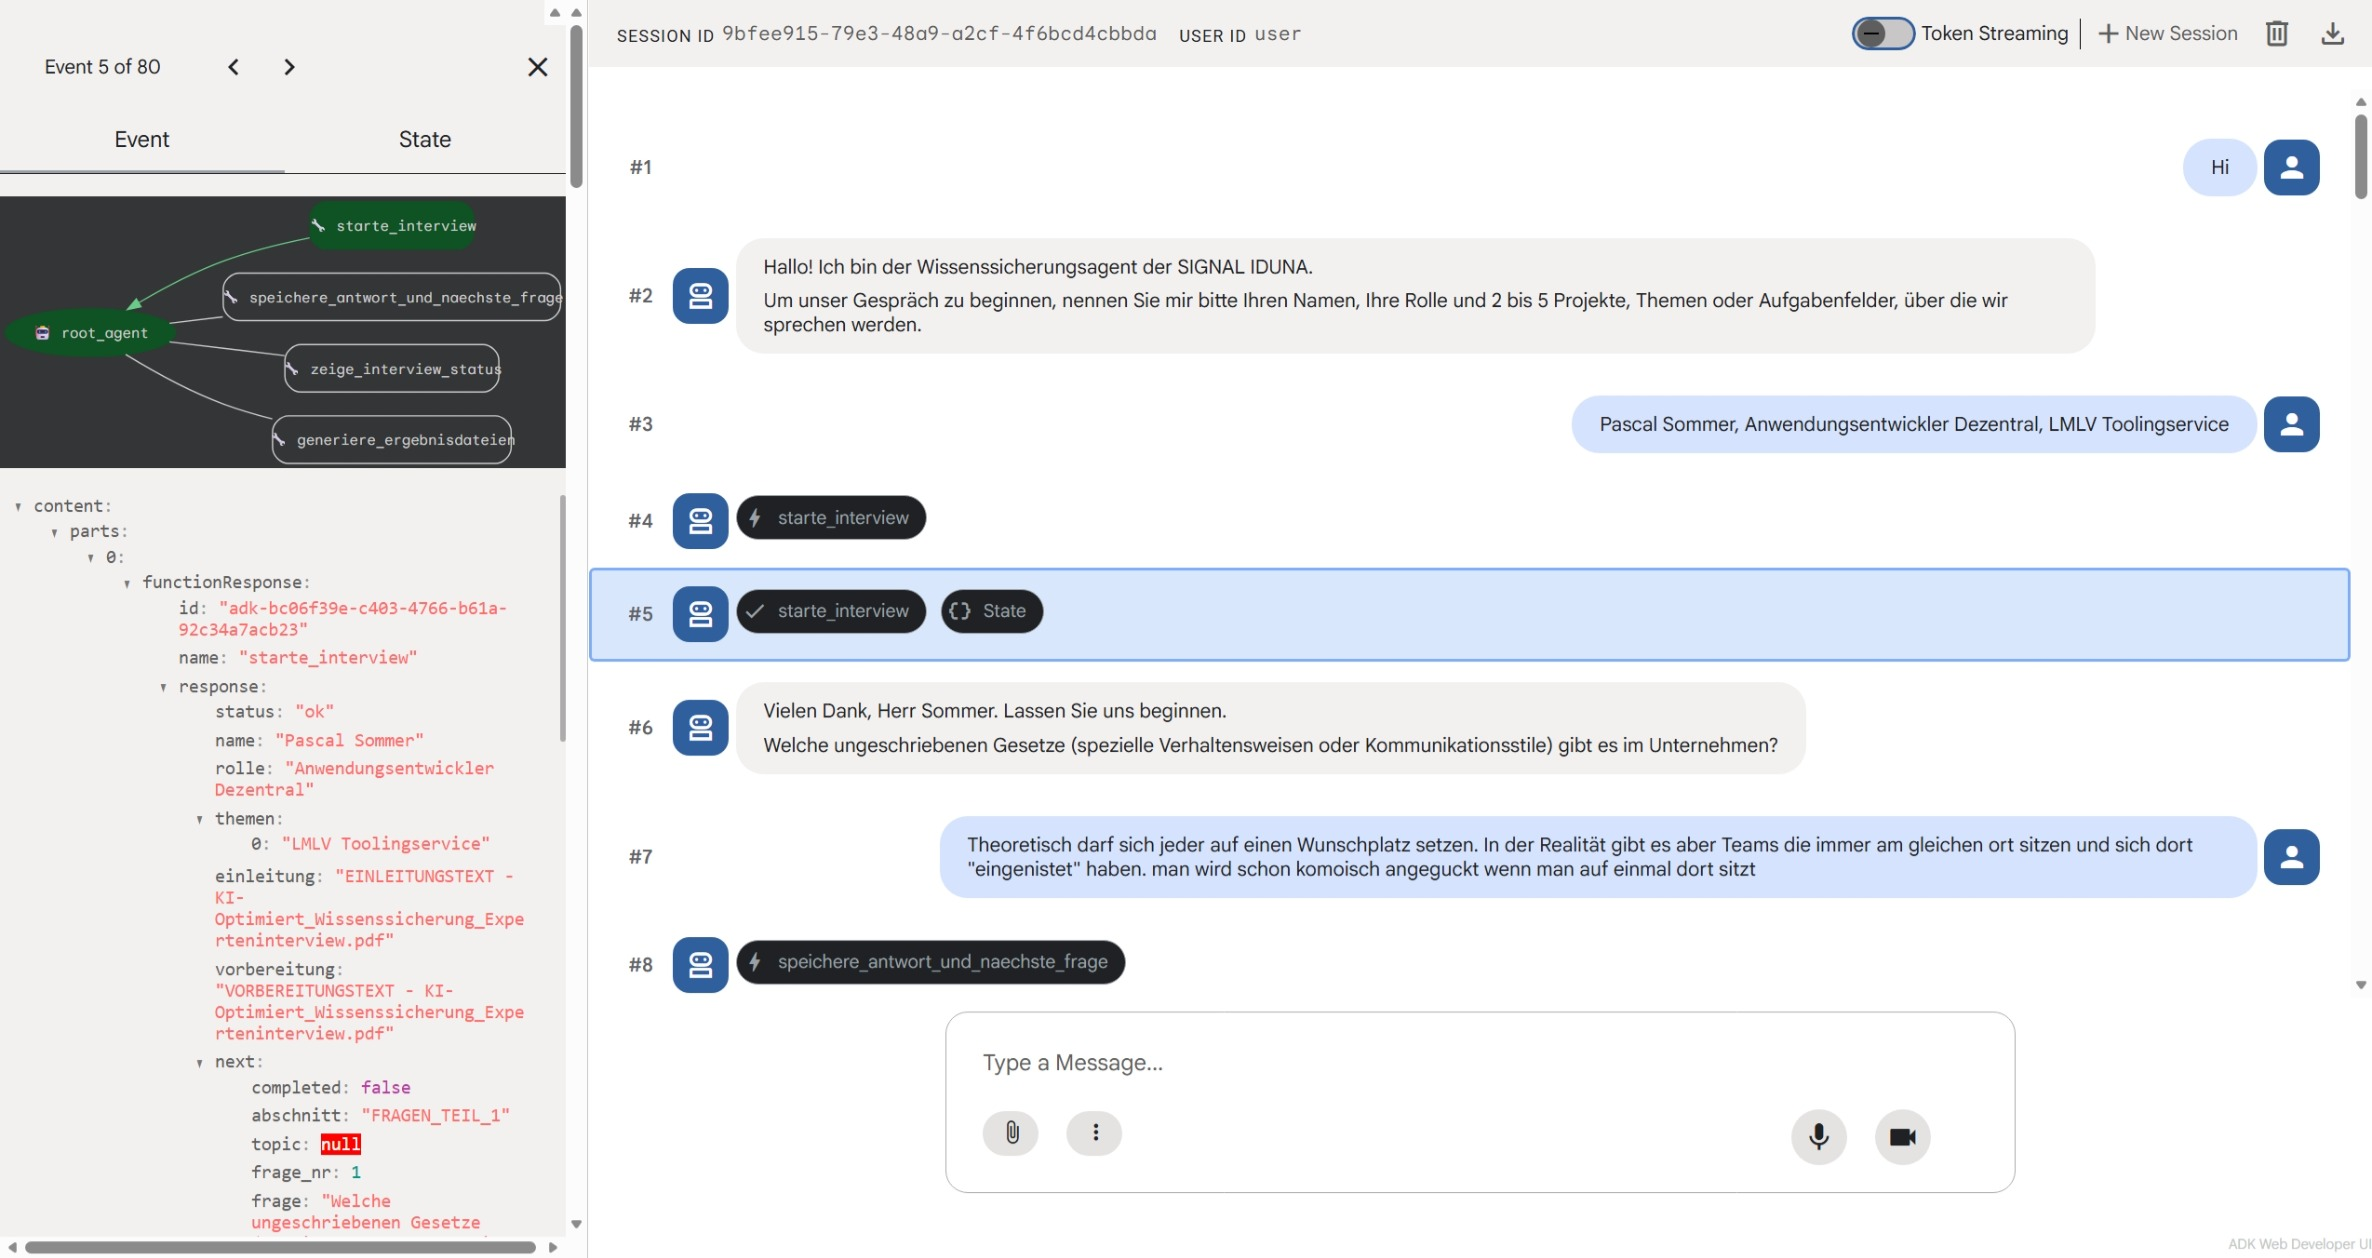
\includegraphics[
        width=0.95\textwidth,
        keepaspectratio
    ]{images/durchlauf1_start.jpeg}
    \caption{Interviewstart in der \glslink{adk}{ADK} Web \glslink{ui}{UI}}
    \label{fig:adk_web_ui_interviewstart}
\end{figure}

\begin{figure}[H]
    \centering
    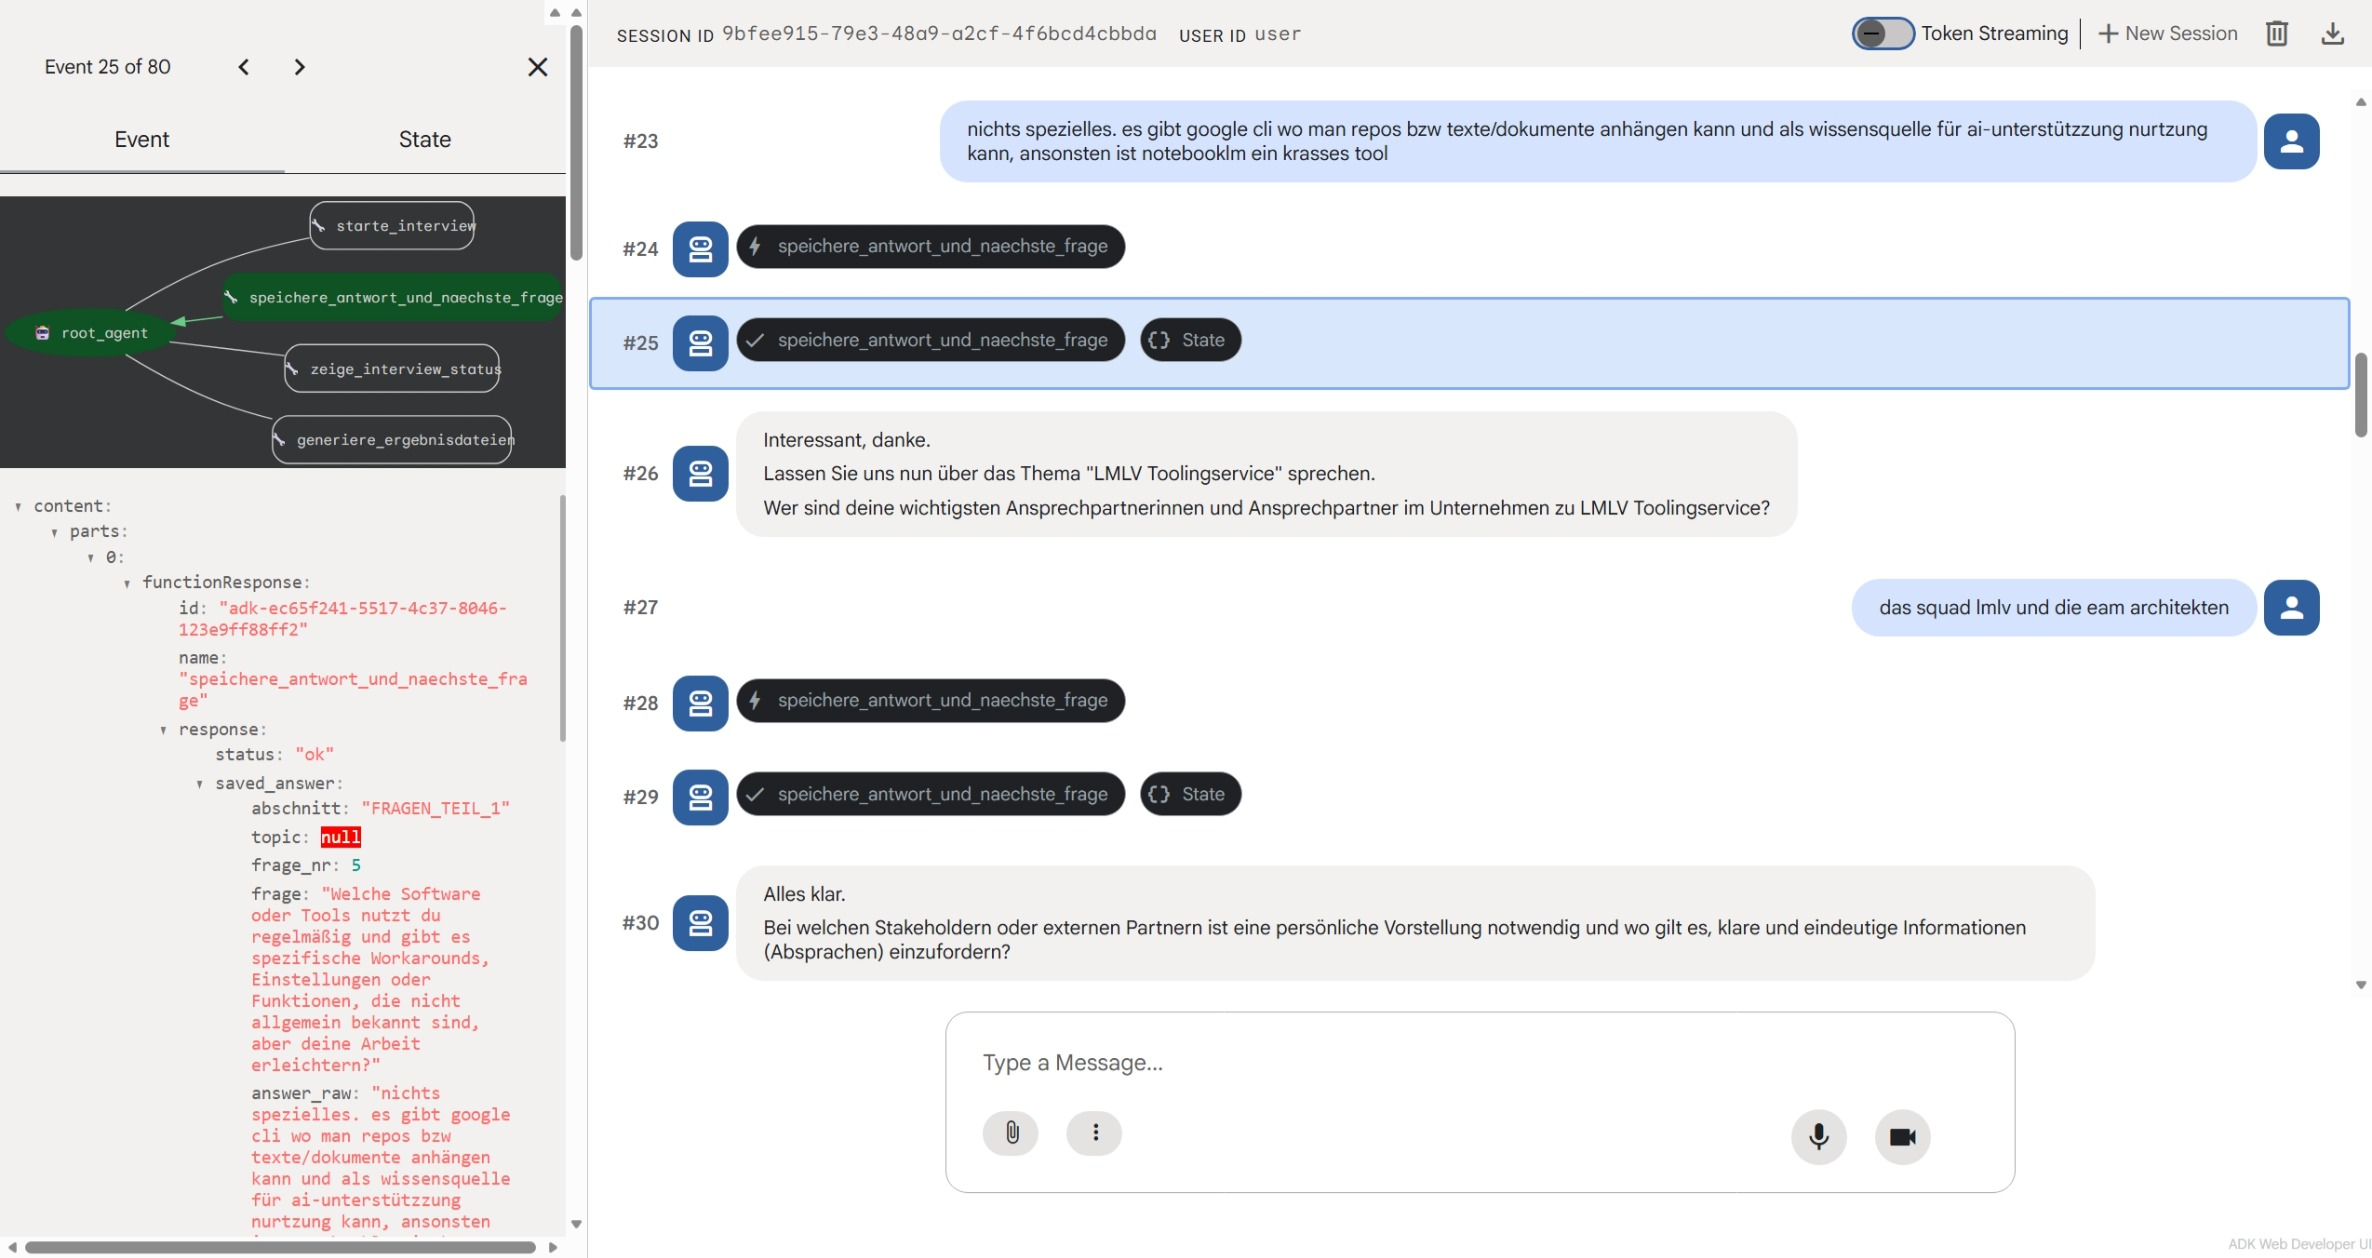
\includegraphics[
        width=0.95\textwidth,
        keepaspectratio
    ]{images/durchlauf1_switch_to_project.jpeg}
    \caption{Projektwechsel in der \glslink{adk}{ADK} Web \glslink{ui}{UI}}
    \label{fig:adk_web_ui_switch_to_project}
\end{figure}

\begin{figure}[H]
    \centering
    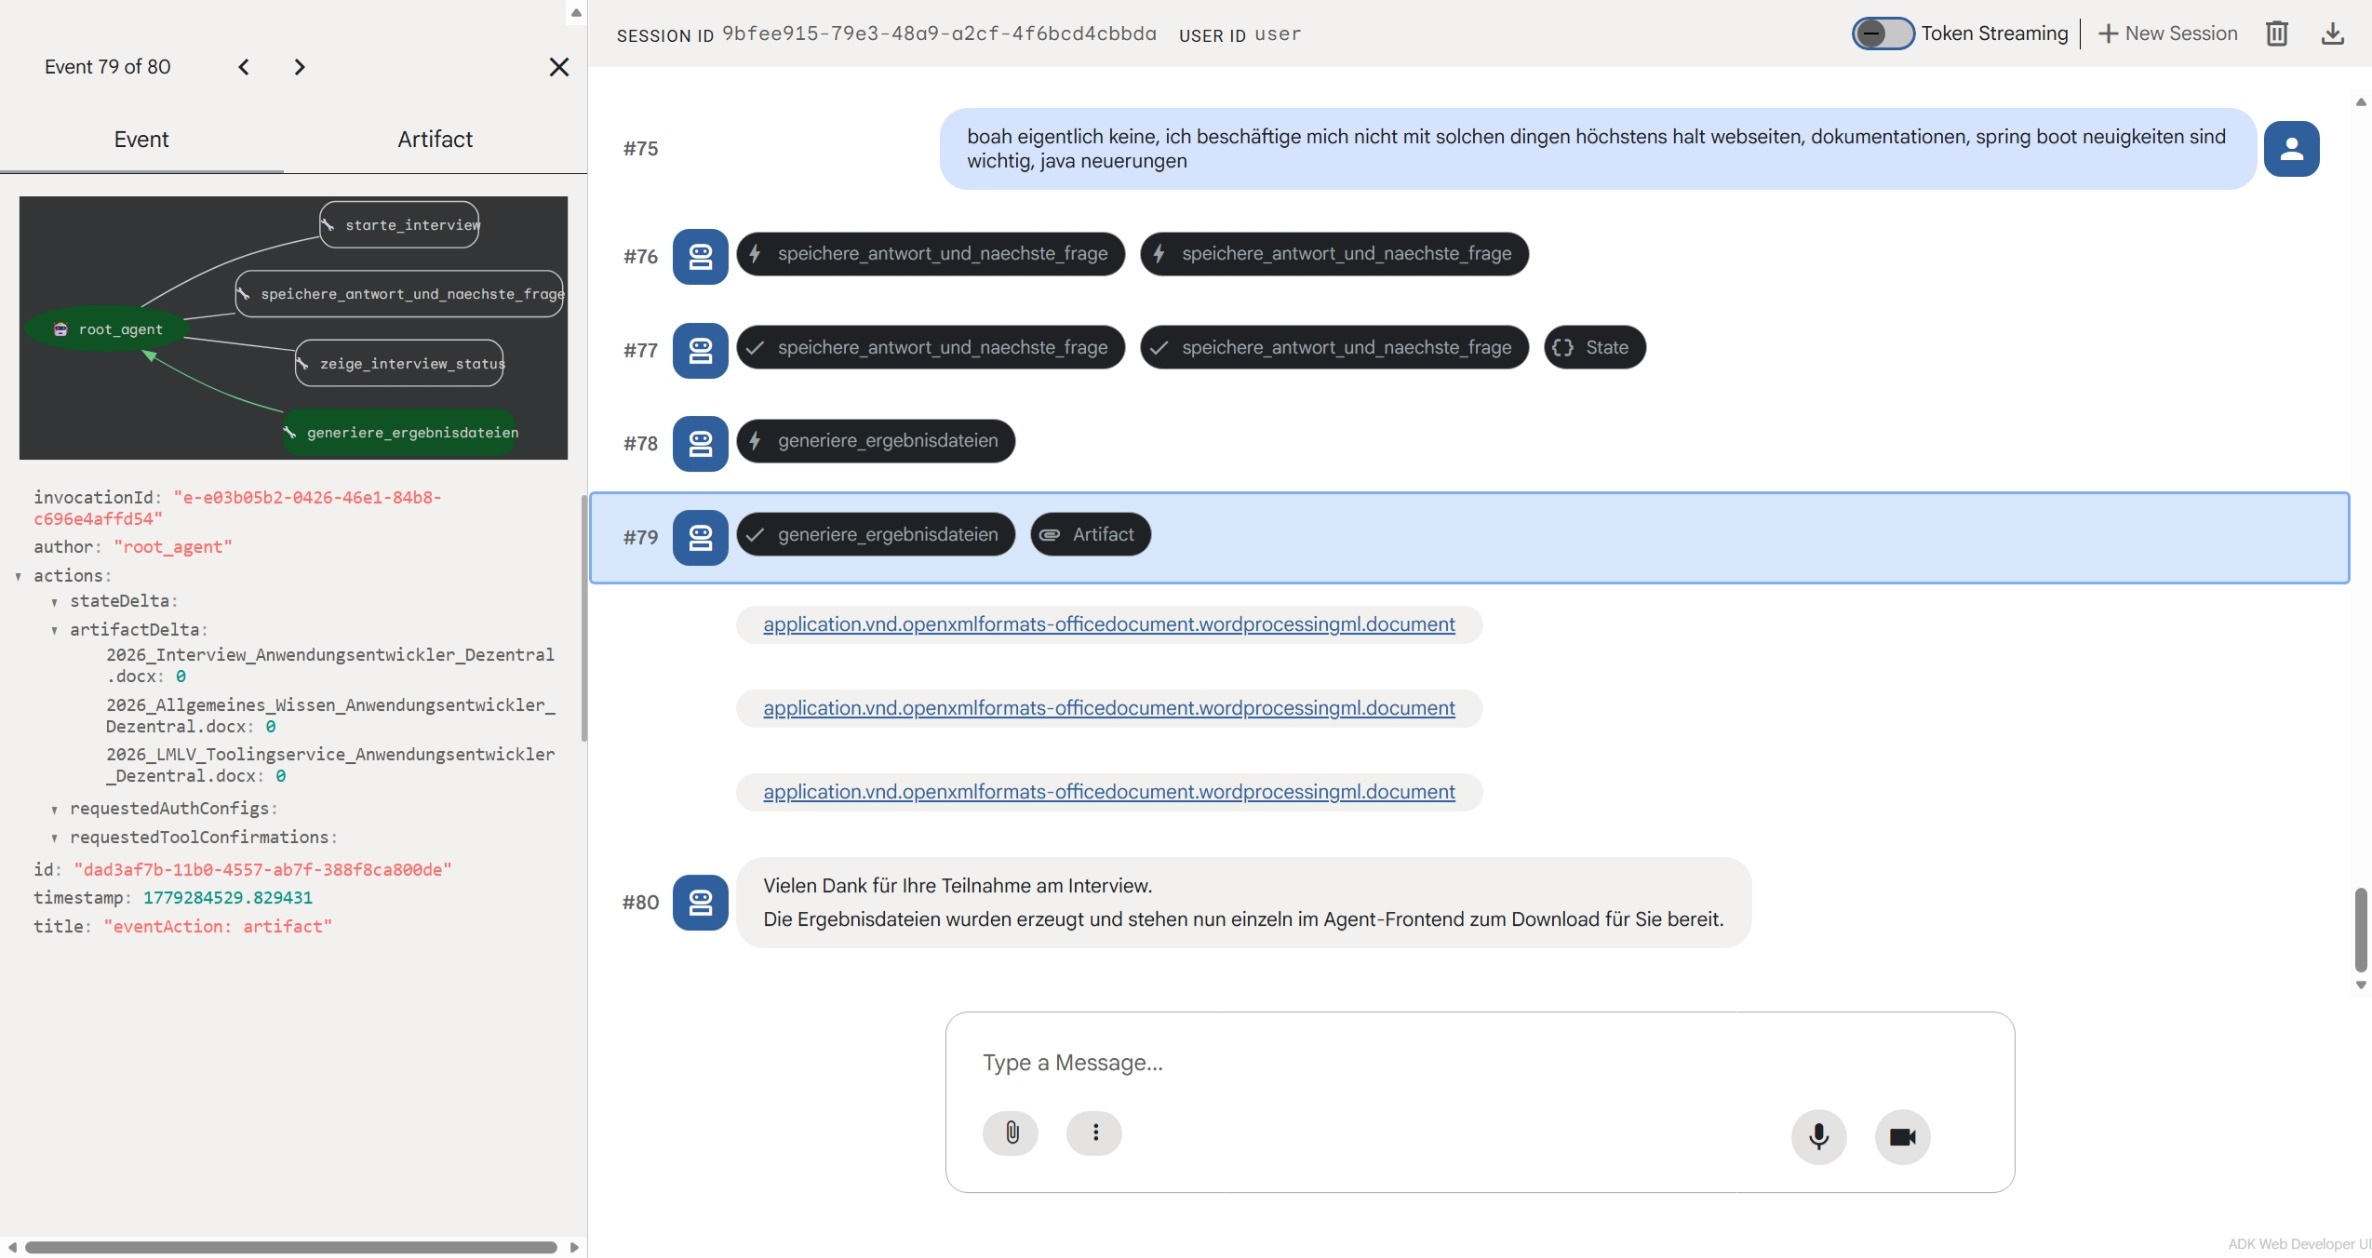
\includegraphics[
        width=0.95\textwidth,
        keepaspectratio
    ]{images/durchlauf2_dokumentenbereitstellung.jpeg}
    \caption{Dokumentenbereitstellung in der \glslink{adk}{ADK} Web \glslink{ui}{UI}}
    \label{fig:adk_web_ui_dokumentenbereitstellung}
\end{figure}
%-------------- A16 Screenshots der ADK Web UI

%Bereitstellung der Ergebnisdateien in der ADK Web UI
%-------------- A17 Fachlicher Kriterienkatalog
\newpage
\subsection{Fachlicher Kriterienkatalog}
\label{anhang_kriterienkatalog}

\begin{table}[H]
\centering
\begin{tabularx}{\textwidth}{|L{4.5cm}|Y|L{2.4cm}|}
\hline
\rowcolor{hkblue}
\textcolor{white}{\textbf{Kriterium}} 
& \textcolor{white}{\textbf{Beschreibung}} 
& \textcolor{white}{\textbf{Bewertung}} \\
\hline

\rowcolor{hklight}
Aufrufbarkeit des Agenten 
& Der Agent ist in der Testumgebung erreichbar und kann gestartet werden. 
& Nicht erfüllt \\
\hline

\rowcolor{hklight}
Nachvollziehbarer Interviewstart 
& Der Agent gibt eine Begrüßung aus, erläutert den Zweck des Interviews und beginnt mit den Eingangsfragen. 
& Erfüllt \\
\hline

\rowcolor{hklight}
Vollständiger Interviewablauf 
& Der Agent führt durch den vorgesehenen Interviewleitfaden und bietet die Pflichtfragen an. 
& Erfüllt \\
\hline

\rowcolor{hklight}
Projektbezogene Wissenssicherung 
& Der Agent stellt projekt- oder themenbezogene Fragen für angegebene Themenbereiche. 
& Erfüllt \\
\hline

\rowcolor{hklight}
Strukturierung der Antworten 
& Die Antworten werden nachvollziehbar kategorisiert und für die Ergebnisdateien aufbereitet. 
& Erfüllt \\
\hline

\rowcolor{hklight}
Bereitstellung der Ergebnisdateien 
& Die Ergebnisdateien werden erzeugt und der nutzenden Person zum Download bereitgestellt. 
& Erfüllt \\
\hline

\rowcolor{hklight}
Fachliche Nutzbarkeit 
& Der Ablauf und die erzeugten Dateien sind aus fachlicher Sicht grundsätzlich als Grundlage für die Wissenssicherung geeignet. 
& Erfüllt \\
\hline

\end{tabularx}
\caption{Fachlicher Kriterienkatalog und Abnahmebewertung}
\label{tab:kriterienkatalog_abnahme}
\end{table}
%-------------- A17 Fachlicher Kriterienkatalog

%-------------- A18 Soll-Ist-Vergleich
\newpage
\subsection{Soll-Ist-Vergleich}
\label{anhang_soll-ist-vergleich}

\begin{table}[H]
\centering
\begin{tabularx}{\textwidth}{|L{4.2cm}|Y|L{2.2cm}|}
\hline
\rowcolor{hkblue}
\textcolor{white}{\textbf{Soll-Zustand}} 
& \textcolor{white}{\textbf{Ist-Umsetzung}} 
& \textcolor{white}{\textbf{Bewertung}} \\
\hline

\rowcolor{hklight}
Aufrufbarer Agent in einer Testumgebung 
& Der Agent kann über die \gls{adk} Web \gls{ui}, jedoch nicht in einer separaten Testumgebung, gestartet und getestet werden. 
& Nicht erfüllt \\
\hline

\rowcolor{hklight}
Strukturierter Interviewablauf mit definiertem Fragenkatalog 
& Die Fragen werden aus der Discovery Engine geladen und in der vorgesehenen Reihenfolge gestellt. 
& Erfüllt \\
\hline

\rowcolor{hklight}
Wiederholung projektbezogener Fragen für angegebene Themen 
& Der zweite Fragenteil wird für jedes angegebene Projekt beziehungsweise Thema durchlaufen. 
& Erfüllt \\
\hline

\rowcolor{hklight}
Speicherung und Kategorisierung der Antworten 
& Die Antworten werden mit Frage, Rohantwort, Kurzfassung, Ergebniskategorie und Key-Word im Session State gespeichert. 
& Erfüllt \\
\hline

\rowcolor{hklight}
Erzeugung strukturierter Ergebnisdateien 
& Nach Abschluss des Interviews werden DOCX-Dokumente erzeugt.
& Erfüllt \\
\hline

\rowcolor{hklight}
Bereitstellung der Ergebnisdateien zum Download 
& Die Ergebnisdateien werden über die Artefaktfunktion der \gls{adk} Web \gls{ui} bereitgestellt. 
& Erfüllt \\
\hline

\rowcolor{hklight}
Einhaltung der \gls{mvp}-Abgrenzung 
& Produktivsetzung, automatische Ablage, Sprachschnittstelle und vollständige Konsistenzprüfung wurden nicht umgesetzt. 
& Erfüllt \\
\hline

\end{tabularx}
\caption{Soll-Ist-Vergleich des Projektergebnisses}
\label{tab:soll_ist_vergleich}
\end{table}
%-------------- A18 Soll-Ist-Vergleich

\end{document}